% Final manuscript source. Last source update: 2026-05-14.
\documentclass[11pt]{article}

\usepackage[utf8]{inputenc}
\usepackage[T1]{fontenc}
\usepackage{lmodern}
\usepackage{amsmath, amssymb, amsthm}
\usepackage{geometry}
\geometry{a4paper, margin=1in}
\usepackage{parskip}
\usepackage{natbib}
\usepackage{graphicx}
\graphicspath{{../figures/}{../03_figures/}}
\usepackage{booktabs}
\usepackage{hyperref}
\usepackage{url}
\usepackage{caption}
\usepackage{subcaption}
\usepackage{enumitem}

% Bibliography is managed manually via \begin{thebibliography}.
% A \bibliographystyle command would be silently ignored and is omitted.

\title{Grammar Competition and Contact-Induced Transient Perturbations in the Old-to-Middle English Transition: A Computational Case Study Using the Symmetric Language Dynamical Equation}
\author{
Carlos Manuel Orrego Franco\thanks{ORCID: \href{https://orcid.org/0009-0001-9163-5137}{0009-0001-9163-5137}}\\
Universidad Nacional de Colombia
\and
Juan Carlos Riaño-Rojas\thanks{ORCID: \href{https://orcid.org/0000-0002-5719-2854}{0000-0002-5719-2854}}\\
Universidad Nacional de Colombia
}
\date{\today}

\providecommand{\keywords}[1]{\textbf{Keywords:} #1}

\begin{document}
\maketitle

\begin{abstract}
The transition from Old English to Middle English unfolded amid regional dialect competition, internal change, and sustained Scandinavian contact in parts of England. This paper asks whether such contact can be represented, cautiously and qualitatively, as a temporary perturbation in grammar competition. We implement the fully symmetric language dynamical equation analyzed by \citet{mitchener2003bifurcation}, in which population frequencies of idealized grammars evolve under communicative selection and imperfect learning. The case study uses four Old English dialectal components---West Saxon, Mercian, Northumbrian, and Kentish---and introduces an idealized Old Norse component during a contact phase. Five scenarios compare a no-contact baseline with conservative, moderate, strong-contact, and canonical Mitchener parameter regimes, varying learning fidelity $q$, average intelligibility $a$, and the Old Norse contact fraction. Numerical integration with adaptive Runge--Kutta methods is evaluated through frequency trajectories, normalized entropy, raw concentration $M_2$, dimension-normalized concentration $C_n$, and transient displacement integrals relative to the no-contact baseline. Across the historically motivated parameter portfolio, contact produces measurable transient displacement toward more distributed states, but not a different long-run attractor. Ablation runs separate the effect of reduced learning fidelity from the effect of introducing a fifth component. The study is exploratory and methodological: it does not reconstruct demographic history or claim that Old Norse contact caused Middle English simplification, but shows how an existing dynamical model can formalize and test qualitative hypotheses about contact and learning.
\end{abstract}

\keywords{language dynamics; historical linguistics; Old English; Middle English; Old Norse; transient perturbation; replicator--mutator dynamics; computational modeling; language contact}

\section{Introduction}

The transition from Old English to Middle English is one of the central episodes in the history of English. It involved large-scale changes in morphology, syntax, lexical composition, and regional variation. Among the historical forces usually discussed are internal developments, dialectal variation, Scandinavian contact in the Danelaw, and later Norman French influence. The present paper focuses only on a deliberately narrow question: how can an existing dynamical-systems model of language competition be used to explore the qualitative effect of a temporary contact-like perturbation in learning conditions?

The mathematical starting point is the language dynamical equation developed by \citet{komarova2001grammar} and analyzed in detail by \citet{mitchener2003bifurcation}. Mitchener studies the fully symmetric case, where all grammars are interchangeable in the sense that cross-grammar intelligibility is represented by a single parameter. In that setting, he rigorously locates fixed points, analyzes their stability, and describes bifurcation scenarios as the reliability of language learning changes.

Crucially, \citet[p.~284]{mitchener2003bifurcation} explicitly suggests the transition from Old English to Middle English as a motivating historical case: Scandinavian speech may have introduced enough linguistic noise to reduce learning reliability in a way that could matter for the stability of competing grammars. This paper does not claim to introduce a new mathematical model. Instead, it operationalizes that suggestion as a reproducible computational case study. The contribution is therefore methodological and exploratory: we define historically interpretable scenarios, simulate the symmetric language dynamical equation across contact phases, and evaluate how sensitive the resulting dynamics are to assumptions about learning fidelity, average intelligibility, and the idealized strength of the Old Norse contact component.

The scope of the claim is intentionally limited. The model tracks frequencies of idealized grammatical systems, not specific morphosyntactic features. It cannot, by itself, prove that Old Norse caused the morphological simplification of Middle English or explain the Old-to-Middle English transition. Rather, it provides a controlled mathematical environment in which one can ask how contact-driven reductions in learning fidelity and contact-component insertion affect transient trajectories in grammar competition.

\section{Related Work}

Mathematical approaches to language change have long used tools from evolutionary dynamics, learning theory, and population-level modeling. \citet{niyogi1997dynamical} proposed a dynamical-systems account of language change in a population of learners. \citet{komarova2001grammar} introduced an evolutionary model of grammar acquisition combining communicative fitness and imperfect learning. Other influential language-competition models include the language-death model of \citet{abramsstrogatz2003language} and extensions incorporating interlinguistic similarity \citep{mira2005interlinguistic}. Broader reviews of social and cultural dynamics locate such models within the statistical-physics tradition \citep{castellano2009statistical}. Mitchener's later analysis provides a complete bifurcation study of the fully symmetric version of the Komarova--Niyogi--Nowak model \citep{mitchener2003bifurcation}.

The present work is closest to Mitchener's fully symmetric language dynamical equation. The model combines a replicator-like selection term with mutation-like learning error, resembling quasispecies dynamics \citep{eigen1971selforganization}. In the symmetric case, learning reliability $q$ becomes the main bifurcation parameter: low values of $q$ favor incoherent equilibria, while high values can support coherent equilibria dominated by one grammar.

A related but distinct line of work applies learning-theoretic models to historical English. \citet{niyogi2009proper} discuss language acquisition and change in a population setting and explicitly model aspects of the evolution of Middle English. Their framework differs from the present one: the focus here is not to replicate the same empirical model, but to explore the behavior of Mitchener's symmetric replicator--mutator system under Old-English-inspired historical scenarios.

More recent work on language contact and change includes models of contact-induced bifurcation and sociolinguistic population dynamics \citep{kauhanen2021replicator,kauhanen2022bifurcation}. These studies motivate the idea that contact conditions can alter the qualitative stability of linguistic systems, although they use different modeling assumptions. Earlier extensions of the language-dynamical tradition also consider competitive exclusion, coexistence, and game dynamics with learning \citep{mitchenernowak2003competitive,mitchener2007game}. Historical and contact-linguistic scholarship provides the empirical background against which any Old English--Old Norse modelling claim must be read \citep{thomasonkaufman1988contact,townend2002language,pons-sanz2013lexical,dawson2003defining,warner2017english}. Work on sociolinguistic typology and historical corpus linguistics provides methodological context for linking social structure and change, but is not used here as direct evidence for Old English--Old Norse contact \citep{walkden2023sociolinguistic}. The present study should therefore be read as a computational bridge between the symmetric language dynamical equation and a historically inspired case study, not as a replacement for corpus-based historical linguistics.

\section{The Symmetric Language Dynamical Equation}

Consider a population in which each individual uses one of $n$ candidate grammatical systems $G_1,\ldots,G_n$. Let $x_j(t)$ denote the proportion of the population using grammar $G_j$ at time $t$, with
\[
    x_j(t)\geq 0, \qquad \sum_{j=1}^n x_j(t)=1.
\]
Thus the state vector $x(t)$ lies in the simplex $S_n$.

Following \citet{mitchener2003bifurcation}, the communicative fitness of grammar $G_i$ is defined by
\begin{equation}
F_i(x)=\sum_{k=1}^n \frac{A_{ik}+A_{ki}}{2}x_k,
\end{equation}
where $A_{ik}$ represents the probability that a sentence produced by a speaker of $G_i$ can be parsed by a speaker of $G_k$. The average fitness is
\begin{equation}
\phi(x)=\sum_{k=1}^n F_k(x)x_k.
\end{equation}

Learning is represented by a row-stochastic matrix $Q$, where $Q_{ij}$ is the probability that a teacher using $G_i$ produces a learner using $G_j$. The general language dynamical equation is
\begin{equation}
\dot{x}_j = \sum_{i=1}^n F_i(x)x_iQ_{ij} - \phi(x)x_j.
\label{eq:general-lde}
\end{equation}
Because $Q$ is row-stochastic, the total population mass is conserved:
\[
\frac{d}{dt}\sum_j x_j = 0.
\]
Moreover, if $x_j=0$, the right-hand side is non-negative, so the positive simplex is invariant.

\subsection{The fully symmetric case}

The fully symmetric model assumes
\begin{equation}
A =
\begin{pmatrix}
1 & a & \cdots & a \\
a & 1 & \cdots & a \\
\vdots & \vdots & \ddots & \vdots \\
a & a & \cdots & 1
\end{pmatrix},
\qquad
Q =
\begin{pmatrix}
q & u & \cdots & u \\
u & q & \cdots & u \\
\vdots & \vdots & \ddots & \vdots \\
u & u & \cdots & q
\end{pmatrix},
\qquad
u=\frac{1-q}{n-1}.
\end{equation}
Here $a$ represents average intelligibility between different grammars, while $q$ represents the probability of faithful learning. Under these assumptions, \citet{mitchener2003bifurcation} obtains the reduced equation
\begin{equation}
\dot{x}_j = (1-a)\left[(q-u)x_j^2 + uM_2 - x_jM_2\right] - aunx_j + au,
\label{eq:symmetric-lde}
\end{equation}
where
\begin{equation}
M_2=\sum_{i=1}^n x_i^2.
\end{equation}

Mitchener's analysis shows that the model can converge either to incoherent equilibria, where several grammars coexist, or coherent equilibria, where one grammar dominates. The present study uses this reduced equation as the computational object of study.

\subsection{Local stability of the uniform equilibrium}

The stability threshold is important for interpreting the simulations below. Linearizing the fully symmetric system around the uniform equilibrium gives the tangential eigenvalue
\begin{equation}
\lambda
=
\frac{1-a}{n}\,[2(q-u)-1]
-
aun,
\qquad
u=\frac{1-q}{n-1}.
\label{eq:uniform-eigenvalue}
\end{equation}
The critical fidelity at which the uniform equilibrium changes local stability is
\begin{equation}
q_c(a,n)
=
\frac{a n^2+(1-a)(n+1)}
{2n(1-a)+a n^2}.
\label{eq:critical-q}
\end{equation}
For $n=4$, this reduces to
\begin{equation}
q_c(a,4)=\frac{5+11a}{8(1+a)}.
\label{eq:critical-q-n4}
\end{equation}
Thus $q_c(0.80,4)\approx 0.9583$ and $q_c(0.75,4)\approx 0.9464$. Since the historically motivated scenarios use $q_1=0.90$, they begin below the threshold required to support local instability of the uniform equilibrium in these high-$a$ regimes. They therefore should not be interpreted as showing that contact destabilizes a previously coherent equilibrium. The canonical comparison with $a=0.50$ has $q_c(0.50,4)=0.875$, placing $q_1=0.90$ closer to Mitchener's coherent-equilibrium regime; it is retained as a methodological comparison rather than as a historical calibration.

\section{Historical Parameterization}
\label{sec:historical-parameterization}

The historical parameterization used in this study is exploratory. It is not a demographic reconstruction of early medieval England. The variables $x_j$ are interpreted as idealized population-level weights for grammatical or dialectal systems, not directly observed proportions of speakers. Likewise, the parameters $q$ and $a$ are not measured historical quantities. They are scenario parameters introduced to probe the qualitative behavior of the model.

We consider four Old English dialectal components:
\begin{itemize}[noitemsep]
    \item $G_1$: West Saxon,
    \item $G_2$: Mercian,
    \item $G_3$: Northumbrian,
    \item $G_4$: Kentish.
\end{itemize}
During the contact phase, a fifth component is introduced:
\begin{itemize}[noitemsep]
    \item $G_5$: Old Norse / Anglo-Scandinavian contact component.
\end{itemize}

The following evidence supports the parameterization, though it must remain explicitly provisional. Several useful claims are supported only indirectly in the current evidence table, for example through secondary summaries or through sources cited by other works. For this reason, the values below are implemented as sensitivity scenarios rather than as historical estimates. The strongest evidence concerns written standardization and literary prestige; the weakest evidence concerns numerical values for learning fidelity and mutual intelligibility.

Late West Saxon is treated as a proxy for written prestige and manuscript standardization, especially in connection with the late Old English / Winchester written tradition \citep{gneuss1972standard,hofstetter1988winchester,gretsch2001winchester}. This modelling choice does not imply that West Saxon was demographically dominant. It only reflects the disproportionate role of West Saxon in the surviving written record. Mercian is included with comparable weight because the Anglian Midlands are commonly treated as central to later English developments, even though the Old English textual record does not preserve Mercian material in direct proportion to its likely territorial and sociolinguistic relevance \citep{hogg1992cambridge,baugh2012history}. Northumbrian is assigned an intermediate initial weight because of its early cultural importance and later documentary disruption. Kentish is assigned a lower weight because of its more geographically restricted role, although this should not be interpreted as evidence that Kentish is linguistically irrelevant.

The Old Norse component should also be interpreted cautiously. The Danelaw and related Anglo-Scandinavian settlement provide historical motivation for a contact phase, but they do not yield a direct numerical estimate of the proportion of Old Norse speakers. Archaeological and historical work has proposed estimates on the order of 20,000--35,000 Scandinavian settlers in some reconstructions \citep{kershawroyvik2016people}, while more recent work emphasizes that the Danelaw should not be treated as a simple, unified demographic block \citep{raffield2020danelaw}. Philological work on Anglo-Scandinavian contact further shows that contact effects must be studied through specific textual, lexical, and sociolinguistic evidence rather than through a single aggregate parameter \citep{townend2002language,pons-sanz2013lexical}. In the model, the Old Norse fraction is therefore a contact-intensity parameter rather than a literal population share.

The parameter $q$ represents learning fidelity. During the contact phase, lower values of $q$ are used to model a noisier learning environment, where children may receive less consistent cues from a multilingual or multidialectal input distribution. This interpretation is consistent with the mechanism proposed by \citet{mitchener2003bifurcation}, but the numerical values of $q$ are heuristic. Contact is treated here as a potential accelerator of ongoing internal changes rather than as a single external cause \citep{dawson2003defining,warner2017english}, and the simulations therefore test contact as a temporary perturbation, not as a proof of causation.

Likewise, $a$ is treated as an average cross-grammar intelligibility parameter. Work on Old Norse--Old English contact is relevant because it discusses linguistic relations and possible mutual intelligibility between speakers of the two related Germanic languages \citep{townend2002language}. However, this does not justify a single measured value of $a$. Because the fully symmetric model cannot represent pairwise differences in intelligibility among West Saxon, Mercian, Northumbrian, Kentish, and Old Norse, $a$ is varied across scenarios rather than fixed as a historical fact.

\subsection{Evidence table and modelling implications}

Table~\ref{tab:evidence} summarizes the current source-based interpretation. The entries should be read as modelling justifications, not measurements.

\begin{table}[h]
\centering
\caption{Historical evidence, modelling implications, and evidence quality.}
\label{tab:evidence}
\scriptsize
\begin{tabular}{p{0.18\textwidth}p{0.27\textwidth}p{0.28\textwidth}p{0.15\textwidth}}
\toprule
Component / parameter & Source-grounded evidence & Modelling implication & Evidence \\
\midrule
West Saxon & Late West Saxon / Winchester written standard; strong role in manuscript transmission \citep{gneuss1972standard,hofstetter1988winchester,gretsch2001winchester} & High initial literary-prestige weight; not demographic majority & Strong support \\
Mercian & Midlands / Anglian relevance to later English developments \citep{hogg1992cambridge,baugh2012history} & Comparable initial weight to West Saxon in central scenarios & Moderate support \\
Northumbrian & Early cultural importance and later documentary disruption in northern records \citep{hogg1992cambridge,baugh2012history} & Intermediate initial weight; corpus-loss caveat & Moderate support \\
Kentish & More geographically restricted dialectal component \citep{hogg1992cambridge,baugh2012history} & Lower initial weight in most scenarios, not zero relevance & Moderate support \\
Old Norse / Anglo-Scandinavian & Danelaw settlement and Anglo-Scandinavian contact; demographic estimates remain contested \citep{kershawroyvik2016people,raffield2020danelaw} & Contact-intensity component, not literal speaker proportion & Moderate support \\
$q$ during contact & Mixed input/contact may reduce cue consistency; modeled after Mitchener's reliability parameter \citep{mitchener2003bifurcation} & Reduced in contact scenarios; must be sensitivity-tested & Heuristic \\
$a$ & Possible partial OE--ON intelligibility and relatedness, but not identity \citep{townend2002language} & Average intelligibility varied across scenarios & Heuristic \\
\bottomrule
\end{tabular}
\end{table}

\subsection{Scenario design}

The simulations use five exploratory scenarios, summarized in Table~\ref{tab:scenarios}. The values should be treated as historically motivated hypotheses to be refined through source-based work and corpus proxies. The central scenario gives equal initial weight to West Saxon and Mercian, lower weight to Northumbrian, and the smallest weight to Kentish. This choice reflects a cautious compromise between textual prestige, territorial relevance, and the absence of direct demographic data.

\begin{table}[h]
\centering
\caption{Exploratory parameter scenarios. Values are not historical measurements; they define sensitivity regimes. The canonical comparison is a methodological reference point based on Mitchener's commonly illustrated $a=0.5$ regime, not a historically calibrated scenario. In the no-contact scenario, the contact phase retains $q_2 = q_1 = 0.90$ (no reduction in learning fidelity) with $n = 4$ grammars throughout; the ``--'' in column $q_2$ indicates the absence of a contact-phase reduction, not the absence of a phase.}
\label{tab:scenarios}
\begin{tabular}{lccccccccc}
\toprule
Scenario & WS & Merc. & North. & Kent. & $q_1$ & $q_2$ & $q_3$ & $a$ & ON frac. \\
\midrule
Conservative & 0.35 & 0.35 & 0.20 & 0.10 & 0.90 & 0.75 & 0.85 & 0.80 & 0.15 \\
Moderate & 0.35 & 0.35 & 0.20 & 0.10 & 0.90 & 0.65 & 0.80 & 0.80 & 0.25 \\
Strong contact & 0.30 & 0.35 & 0.20 & 0.15 & 0.90 & 0.55 & 0.75 & 0.75 & 0.33 \\
Canonical comparison & 0.35 & 0.35 & 0.20 & 0.10 & 0.90 & 0.60 & 0.80 & 0.50 & 0.33 \\
No contact & 0.35 & 0.35 & 0.20 & 0.10 & 0.90 & -- & 0.90 & 0.80 & 0.00 \\
\bottomrule
\end{tabular}
\end{table}

The contact scenarios are organized into three phases:
\begin{enumerate}[noitemsep]
    \item \textbf{Pre-contact phase}: four Old English dialectal components, high learning fidelity $q_1$.
    \item \textbf{Contact phase}: Old Norse is introduced as an idealized fifth component, and learning fidelity is reduced to $q_2$.
    \item \textbf{Post-contact phase}: the Old Norse component is removed and redistributed among Old English components, while learning fidelity partially recovers to $q_3$.
\end{enumerate}

The no-contact scenario is a counterfactual baseline in which no Old Norse component is introduced and learning fidelity remains at $q_1$ throughout all three phases. To ensure this is a strict four-grammar baseline, the integration uses $n=4$ in all phases; the $G_5$ column is absent rather than initialized at zero, preventing the mutation term from generating a phantom Old Norse component.

\subsection{Phase-transition maps}

The numerical experiments are not a single autonomous ODE on a fixed simplex. They are a hybrid phase system with two discrete transition maps:
\[
S_4 \longrightarrow S_5 \longrightarrow S_4.
\]
Let $x\in S_4$ be the Old English state immediately before contact. At the beginning of the contact phase, the Old Norse component is introduced with contact intensity $\theta$ by
\begin{equation}
\mathcal I_\theta(x)
=
\bigl((1-\theta)x_1,\ldots,(1-\theta)x_4,\theta\bigr)
\in S_5.
\label{eq:introduction-map}
\end{equation}
Here $\theta$ is the ``Old Norse fraction'' in Table~\ref{tab:scenarios}; it is a contact-intensity parameter, not a literal demographic proportion.

At the end of contact, the fifth component is removed and its mass is redistributed among the four Old English components:
\begin{equation}
\mathcal R_\rho(y)
=
\bigl(y_1+\rho_1y_5,\ldots,y_4+\rho_4y_5\bigr)
\in S_4,
\label{eq:redistribution-map}
\end{equation}
where
\[
\rho_i\ge 0,\qquad \sum_{i=1}^4 \rho_i=1.
\]
The main simulations use the neutral uniform rule
\[
\rho_i=\frac{1}{4}.
\]
These maps are not part of the continuous language dynamical equation. They are discrete transitions between phase-specific ODE integrations. Consequently, visible jumps in entropy and concentration diagnostics at the phase boundaries reflect the maps and the change in dimension as well as the subsequent continuous dynamics. Section~\ref{sec:redistribution-sensitivity} reports a simple sensitivity check using proportional redistribution,
\[
\rho_i=\frac{y_i}{\sum_{k=1}^4 y_k}.
\]

\subsection{Interpretive scope}

Several aspects of the model design carry important interpretive limits. The initial West Saxon weight reflects written-prestige assignment in the surviving manuscript record, not a claim about spoken demographic dominance. The Old Norse fraction is a contact-intensity parameter calibrated to historical plausibility rather than a literal population share; similarly, the learning-fidelity values are scenario-dependent heuristics, not empirically measured quantities. The simulations treat contact as one potential perturbation alongside internal change, regional variation, and later external influences, and the results bear on transient model dynamics rather than on the ultimate cause of Middle English morphological simplification. Because the fully symmetric model assigns uniform pairwise intelligibility, the parameter $a$ should be understood as a scenario sensitivity variable rather than a measured linguistic fact about any specific language pair.

\section{Numerical Method}

The initial value problem is
\begin{equation}
\frac{d x}{dt}=f(x;q,a,n),\qquad x(t_0)=x_0,
\end{equation}
where $f$ is defined componentwise by Equation~\eqref{eq:symmetric-lde}. Numerical integration was performed using \texttt{scipy.integrate.solve\_ivp} with the explicit adaptive Runge--Kutta method \texttt{RK45}, tolerances \texttt{rtol}$=10^{-10}$ and \texttt{atol}$=10^{-12}$. The accompanying implementation is the public repository script \texttt{simulation.py}\footnote{All simulation code is publicly available at \url{https://github.com/cmorregof/language_dynamics}. The repository includes the main Python script, dependencies, generated figures, and CSV outputs for the reported tables.}. For each run, the following diagnostics were monitored:
\begin{itemize}[noitemsep]
    \item conservation of mass: $\max_t |\sum_j x_j(t)-1|$;
    \item positivity: $\min_{j,t} x_j(t)$;
    \item normalized entropy:
    \begin{equation}
        H_{\mathrm{norm}}(x)=-\frac{1}{\log n}\sum_{j=1}^n x_j\log x_j;
    \end{equation}
    \item concentration/coherence proxy:
    \begin{equation}
        M_2(x)=\sum_{j=1}^n x_j^2.
    \end{equation}
    \item dimension-normalized concentration:
    \begin{equation}
        C_n(x)=\frac{M_2(x)-1/n}{1-1/n}.
        \label{eq:normalized-concentration}
    \end{equation}
\end{itemize}

Entropy is high when several grammars coexist with comparable weights. The statistic $M_2$ is low near the uniform state and increases as the population concentrates around fewer grammatical systems. Raw $M_2$ remains useful because it appears naturally in the symmetric LDE, but it is dimension-dependent: the uniform minimum is $1/4$ in $S_4$ and $1/5$ in $S_5$. Therefore raw $M_2$ is not the primary metric for comparing concentration across the contact and no-contact trajectories. The normalized statistic $C_n$ is 0 at the uniform state for any $n$ and 1 at a simplex vertex, making it the primary concentration metric for cross-phase comparisons. These quantities do not measure historical linguistic complexity; they measure diversity and concentration in the model state.

\paragraph*{Transient displacement integrals.}
To quantify the cumulative deviation of each contact scenario from the no-contact baseline, scalar diagnostics are defined. Let $[t_0, t_f] = [0, 120]$ denote the full simulation window in model units.\footnote{The time variable $t$ in the symmetric language dynamical equation is dimensionless. No specific mapping to calendar years or linguistic generations is assumed; the model explores qualitative dynamics rather than quantitative historical reconstruction.} For each contact scenario, the absolute difference between its diagnostic trajectory and the corresponding no-contact baseline trajectory is integrated over this window:
\begin{align}
    D_H &= \int_{t_0}^{t_f}
             \bigl|H_{\mathrm{norm,contact}}(t) - H_{\mathrm{norm,no\text{-}contact}}(t)\bigr|
             \,\mathrm{d}t,
    \label{eq:dH} \\
    D_C &= \int_{t_0}^{t_f}
               \bigl|C_{n(t),\mathrm{contact}}(t) - C_{4,\mathrm{no\text{-}contact}}(t)\bigr|
               \,\mathrm{d}t.
    \label{eq:dC}
\end{align}
These integrals summarize how far, and for how long, a contact scenario departs from the no-contact baseline in a single scalar value: a scenario that produces a large instantaneous deviation, or one that produces a smaller but long-lasting deviation, will yield a larger integral. Because all historically motivated scenarios converge to the same final state as the no-contact baseline, $D_H$ and $D_C$ capture the transient geometry of the contact effect rather than any change in the long-run attractor. We also report raw $D_{M_2}$ as a descriptive diagnostic, but it is explicitly labelled as dimension-dependent because the shift from $n=4$ to $n=5$ contributes mechanically to its value. Numerical evaluation uses the trapezoid rule applied to the concatenated time grid, which is identical across all scenarios by construction.

A fixed-step classical RK4 implementation was used to verify convergence: comparing step sizes $h$, $h/2$, and $h/4$ for Phase~1 of the moderate scenario yields a maximum L$_\infty$ error of $1.6 \times 10^{-12}$ at $h=0.1$, confirming fourth-order convergence of the reference RK4 implementation and providing indirect corroboration of the RK45 solution.

\section{Computational Experiments}

The experiments are organized around three questions:
\begin{enumerate}[noitemsep]
    \item How do grammar-frequency trajectories differ between contact and no-contact
          scenarios during and after the contact phase?
    \item How do entropy and dimension-normalized concentration $C_n$ respond to the reduction in learning fidelity
          during contact, and how long does that response persist into the
          post-contact phase?
    \item Across what range of $(a, q_2)$ does the contact-phase perturbation remain
          qualitatively similar to the historically motivated scenarios, and where
          does the model enter a regime with stronger final-state consequences?
\end{enumerate}

\subsection{Temporal trajectories}

Figure~\ref{fig:frequencies} shows the trajectory of the moderate scenario. The vertical dashed lines mark the beginning and end of the contact phase. During contact, the Old Norse component is introduced and the learning reliability parameter is reduced. The interpretation should be qualitative: the figure illustrates how the dynamical system responds to a parameter shock, not how actual speaker populations evolved year by year.

During the contact phase, the four Old English components are displaced from their pre-contact trajectories as the introduced Old Norse component and the reduced learning fidelity jointly increase diversity and reduce concentration. After the contact phase ends and $q$ partially recovers, the Old English components consolidate again. The transient displacement---the departure from the no-contact trajectory and the path taken through state space during the contact phase---is the primary object of interest in the results below, since all scenarios converge to the same near-uniform final state.

\begin{figure}[h]
    \centering
    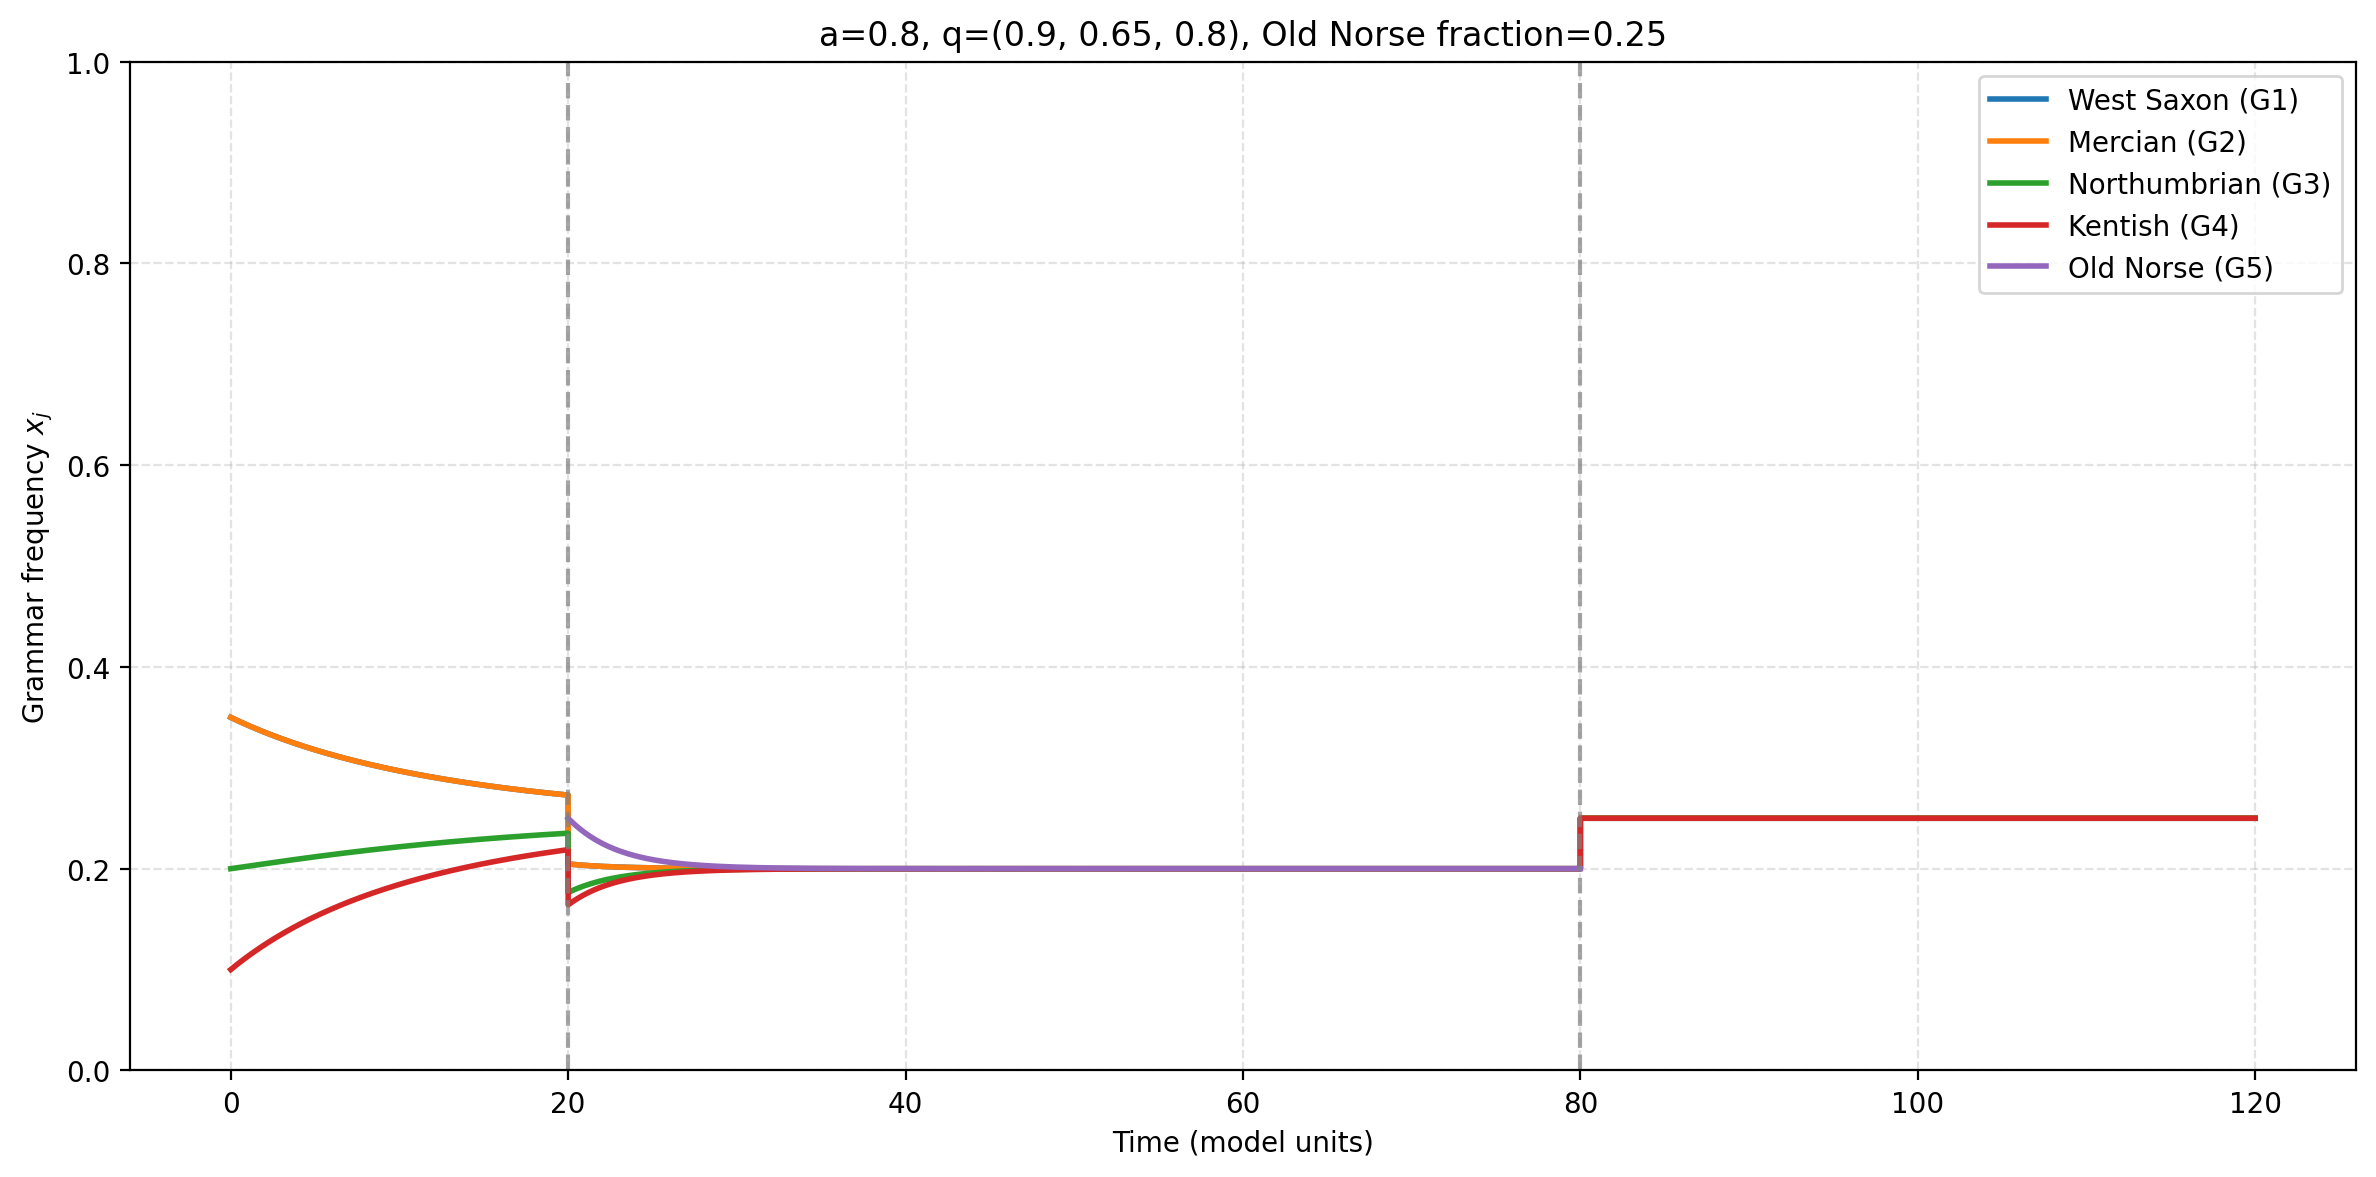
\includegraphics[width=0.85\textwidth]{lde_moderate_frequencies.png}
    \caption{Frequency trajectories in the moderate contact scenario. The Old Norse component is introduced during the contact phase and removed in the post-contact phase.}
    \label{fig:frequencies}
\end{figure}

\subsection{Entropy and normalized concentration}

Figures~\ref{fig:entropy} and~\ref{fig:concentration} show model-state diagnostics for the moderate scenario. In the moderate scenario, normalized entropy rises and $C_n$ falls at the onset of the contact phase, indicating that the system moves toward a more distributed state. This is the expected response to a reduction in learning fidelity: when $q$ decreases, the mutation-like contribution becomes relatively stronger and the system is pulled toward the near-uniform equilibrium. When $q$ partially recovers in the post-contact phase, the system begins to consolidate again. The key observation is that this effect is phase-dependent and transient: in the parameter regime used here, the final state of the system is the same near-uniform configuration regardless of whether contact occurred. The contact phase produces a detour through a more distributed region of state space, not a shift in the long-run attractor.

\begin{figure}[h]
    \centering
    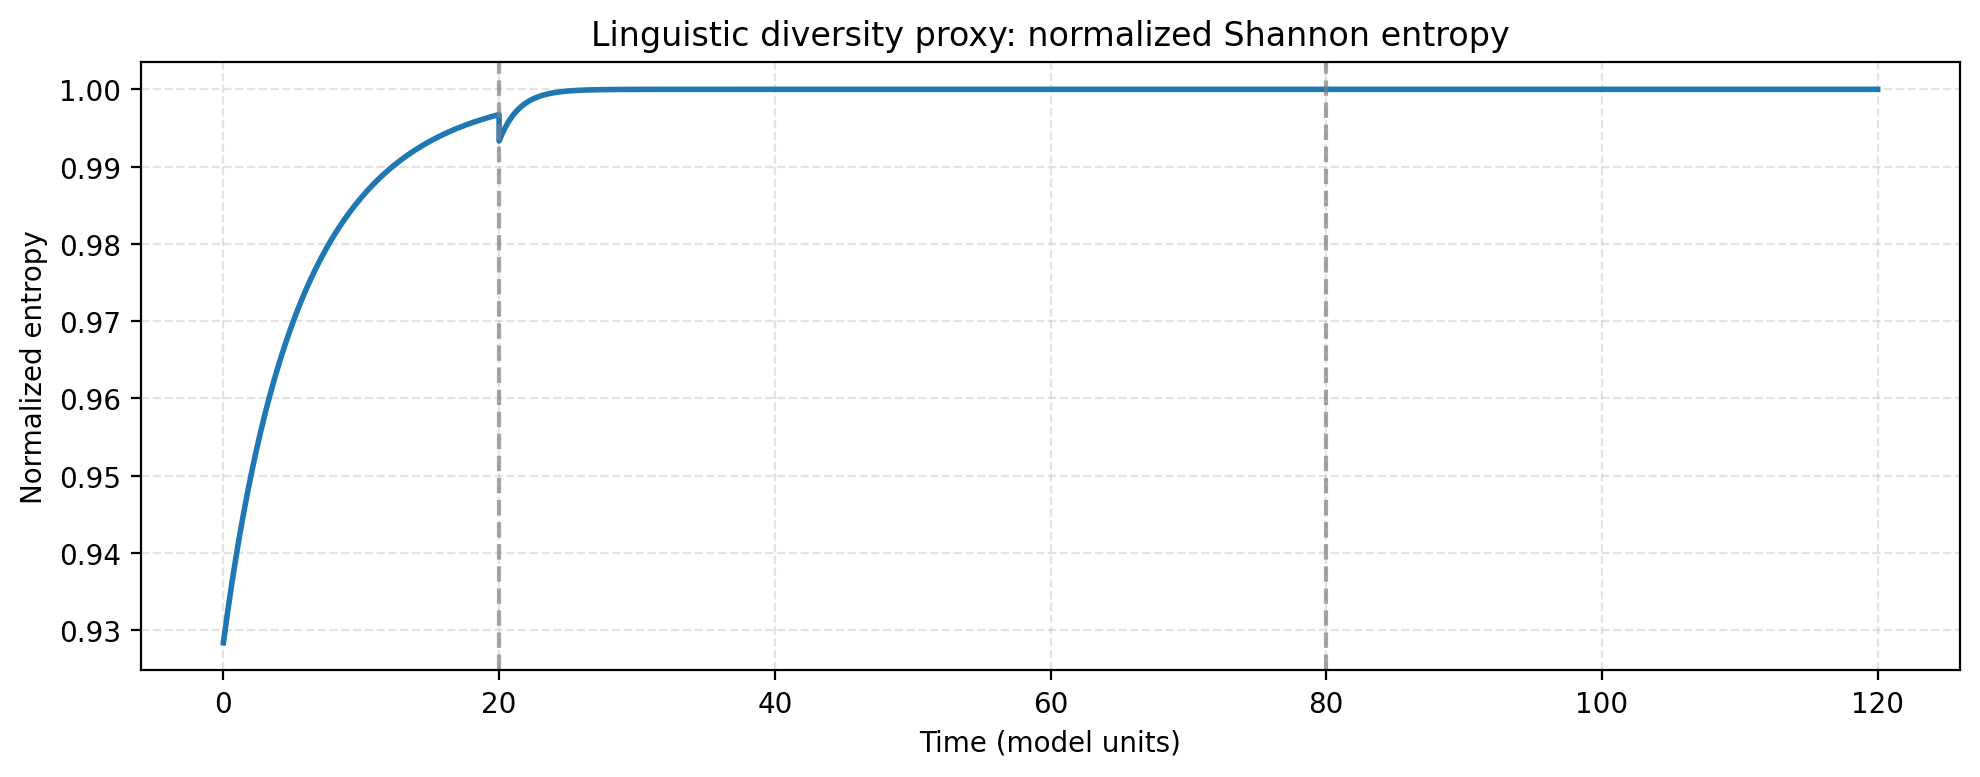
\includegraphics[width=0.85\textwidth]{lde_moderate_diagnostics_entropy.png}
    \caption{Normalized entropy in the moderate contact scenario. Higher values indicate greater diversity among model components. The apparent phase-boundary shifts also reflect the change in model dimension from $n=4$ to $n=5$ and back to $n=4$.}
    \label{fig:entropy}
\end{figure}

\begin{figure}[h]
    \centering
    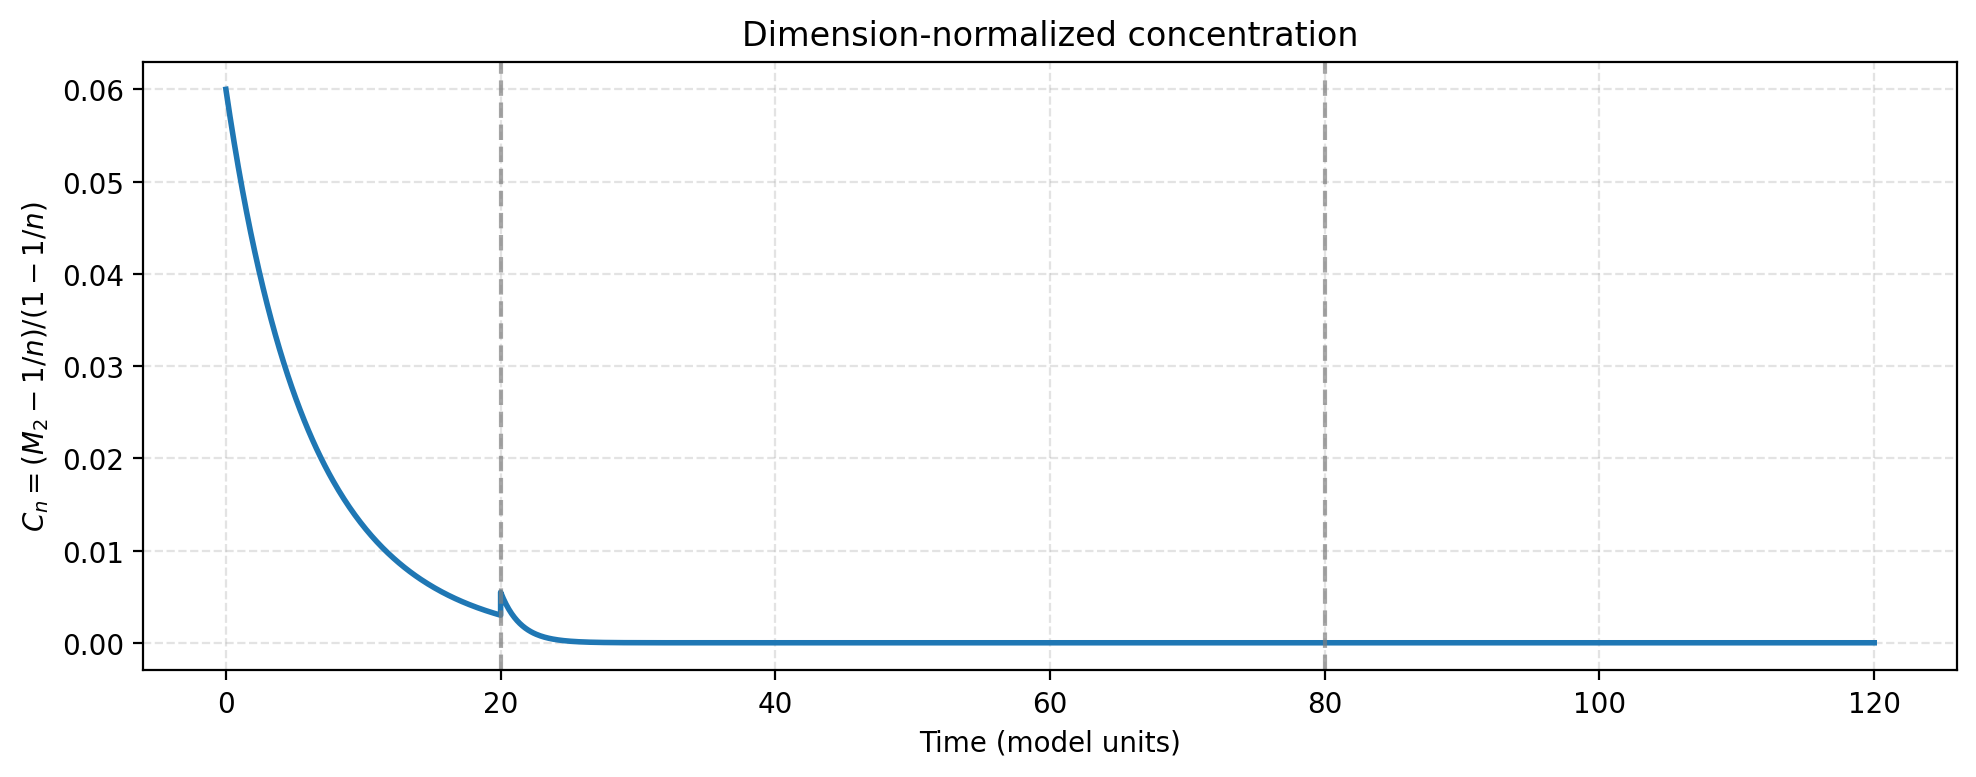
\includegraphics[width=0.85\textwidth]{lde_moderate_diagnostics_concentration.png}
    \caption{Dimension-normalized concentration $C_n$ in the moderate contact scenario. Higher values indicate stronger concentration in fewer components, while $C_n=0$ corresponds to the uniform state in either $S_4$ or $S_5$.}
    \label{fig:concentration}
\end{figure}

\subsection{Scenario comparison}

Scenario comparisons allow us to avoid over-interpreting a single parameter set. Across the contact scenarios, the robust result is a transient elevation of normalized entropy and a corresponding depression of dimension-normalized concentration $C_n$, relative to the no-contact baseline. The depth and duration of this transient response vary with the scenario parameters. Figures~\ref{fig:scenario-entropy} and~\ref{fig:scenario-concentration} show this pattern.

\begin{figure}[h]
    \centering
    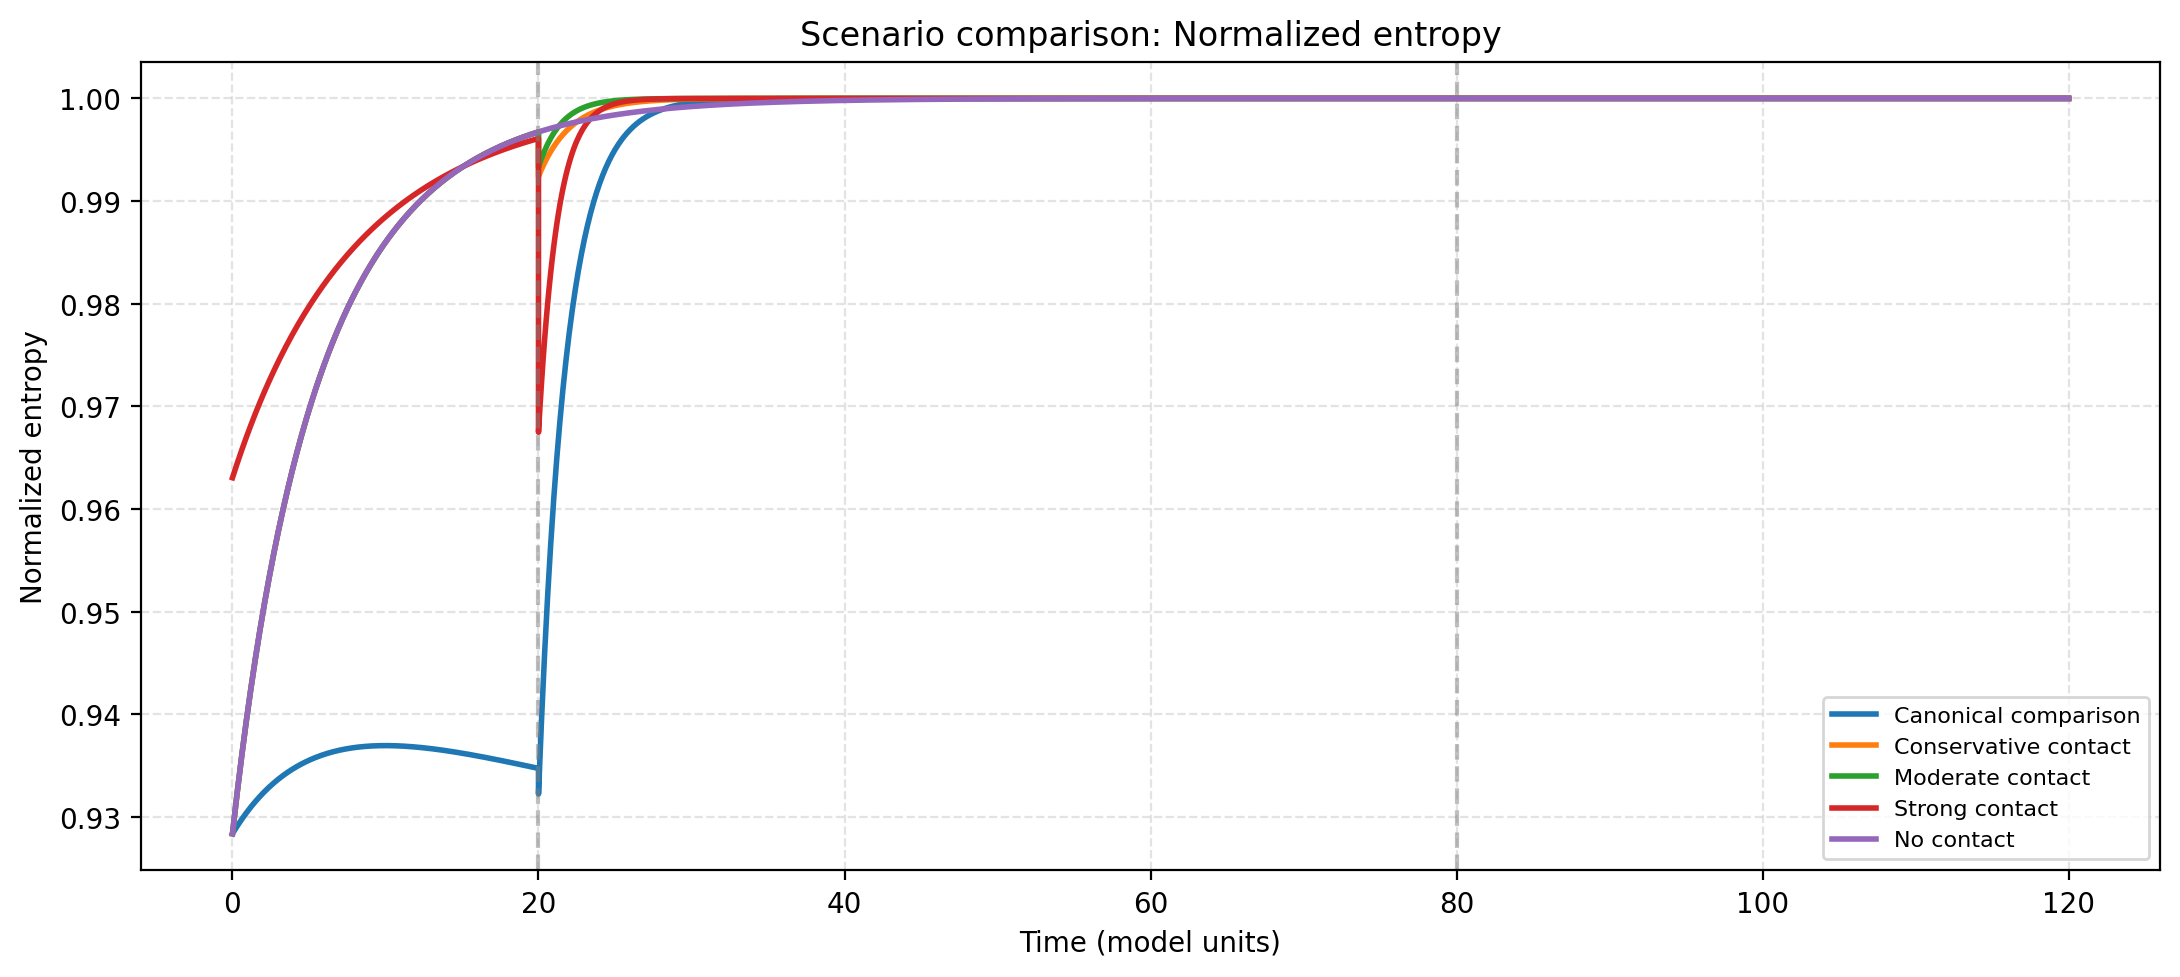
\includegraphics[width=0.85\textwidth]{lde_scenario_entropy.png}
    \caption{Comparison of normalized entropy across exploratory scenarios. Contact scenarios contain a five-component middle phase, whereas the no-contact baseline remains four-dimensional throughout.}
    \label{fig:scenario-entropy}
\end{figure}

\begin{figure}[h]
    \centering
    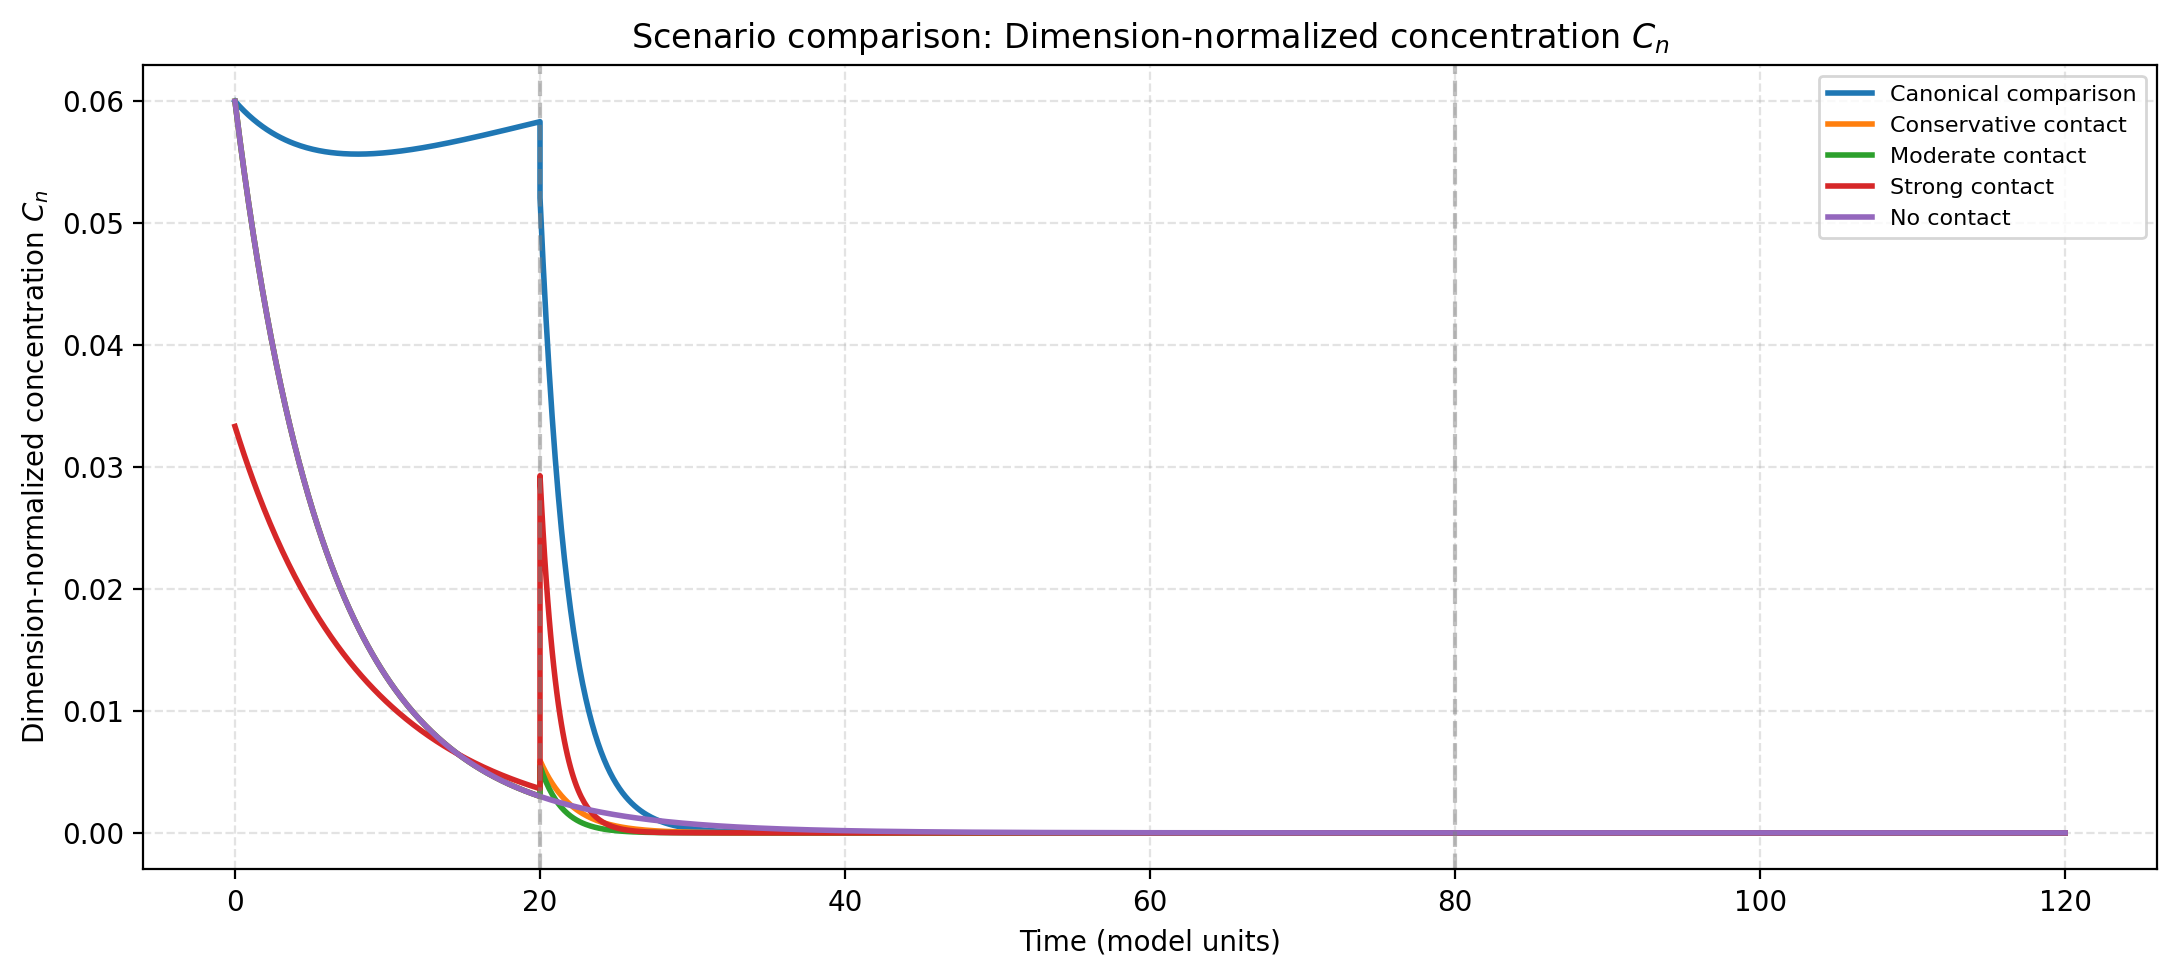
\includegraphics[width=0.85\textwidth]{lde_scenario_concentration.png}
    \caption{Comparison of dimension-normalized concentration $C_n$ across exploratory scenarios. This normalization removes the mechanical shift in the minimum concentration value when the contact scenarios enter the five-component phase.}
    \label{fig:scenario-concentration}
\end{figure}

Table~\ref{tab:numerical-summary} reports final diagnostic values for the scenario portfolio. All scenarios converge to normalized entropy of 1.0, $M_2 = 0.25$, and $C_4=0$, corresponding to the uniform four-component distribution. Final-state divergence is therefore not a feature of this parameter portfolio; the main differences among scenarios are transient and phase-dependent.

\begin{table}[h]
\centering
\caption{Diagnostics for the exploratory scenarios, generated by \texttt{simulation.py}. Final entropy, final $M_2$, and final $C_4$ are endpoint values at $t=120$. Max mass error and minimum component are trajectory-wide extrema across all simulation phases, not final-state values.}
\label{tab:numerical-summary}
\scriptsize
\begin{tabular}{lccccc}
\toprule
Scenario & Final entropy & Final $M_2$ & Final $C_4$ & Max mass error & Min. component \\
\midrule
Canonical comparison & 1.0000 & 0.2500 & 0.0000 & $8.88\times 10^{-16}$ & 0.0909 \\
Conservative contact & 1.0000 & 0.2500 & 0.0000 & $2.22\times 10^{-16}$ & 0.1000 \\
Moderate contact & 1.0000 & 0.2500 & 0.0000 & $3.89\times 10^{-15}$ & 0.1000 \\
Strong contact & 1.0000 & 0.2500 & 0.0000 & $1.17\times 10^{-13}$ & 0.1468 \\
No contact & 1.0000 & 0.2500 & 0.0000 & $2.22\times 10^{-16}$ & 0.1000 \\
\bottomrule
\end{tabular}
\end{table}

Figure~\ref{fig:comparison} provides a direct visual comparison of the no-contact baseline and the moderate contact scenario at the level of individual grammar frequencies. In the no-contact panel, the four Old English dialects drift slowly and monotonically toward the uniform state under constant high learning fidelity. In the contact panel, the same four dialects are visibly displaced during the contact phase before recovering. This comparison makes the transient character of the contact perturbation concrete: the trajectories diverge during the contact window and converge again afterward, ending at the same final state.

\begin{figure}[h]
    \centering
    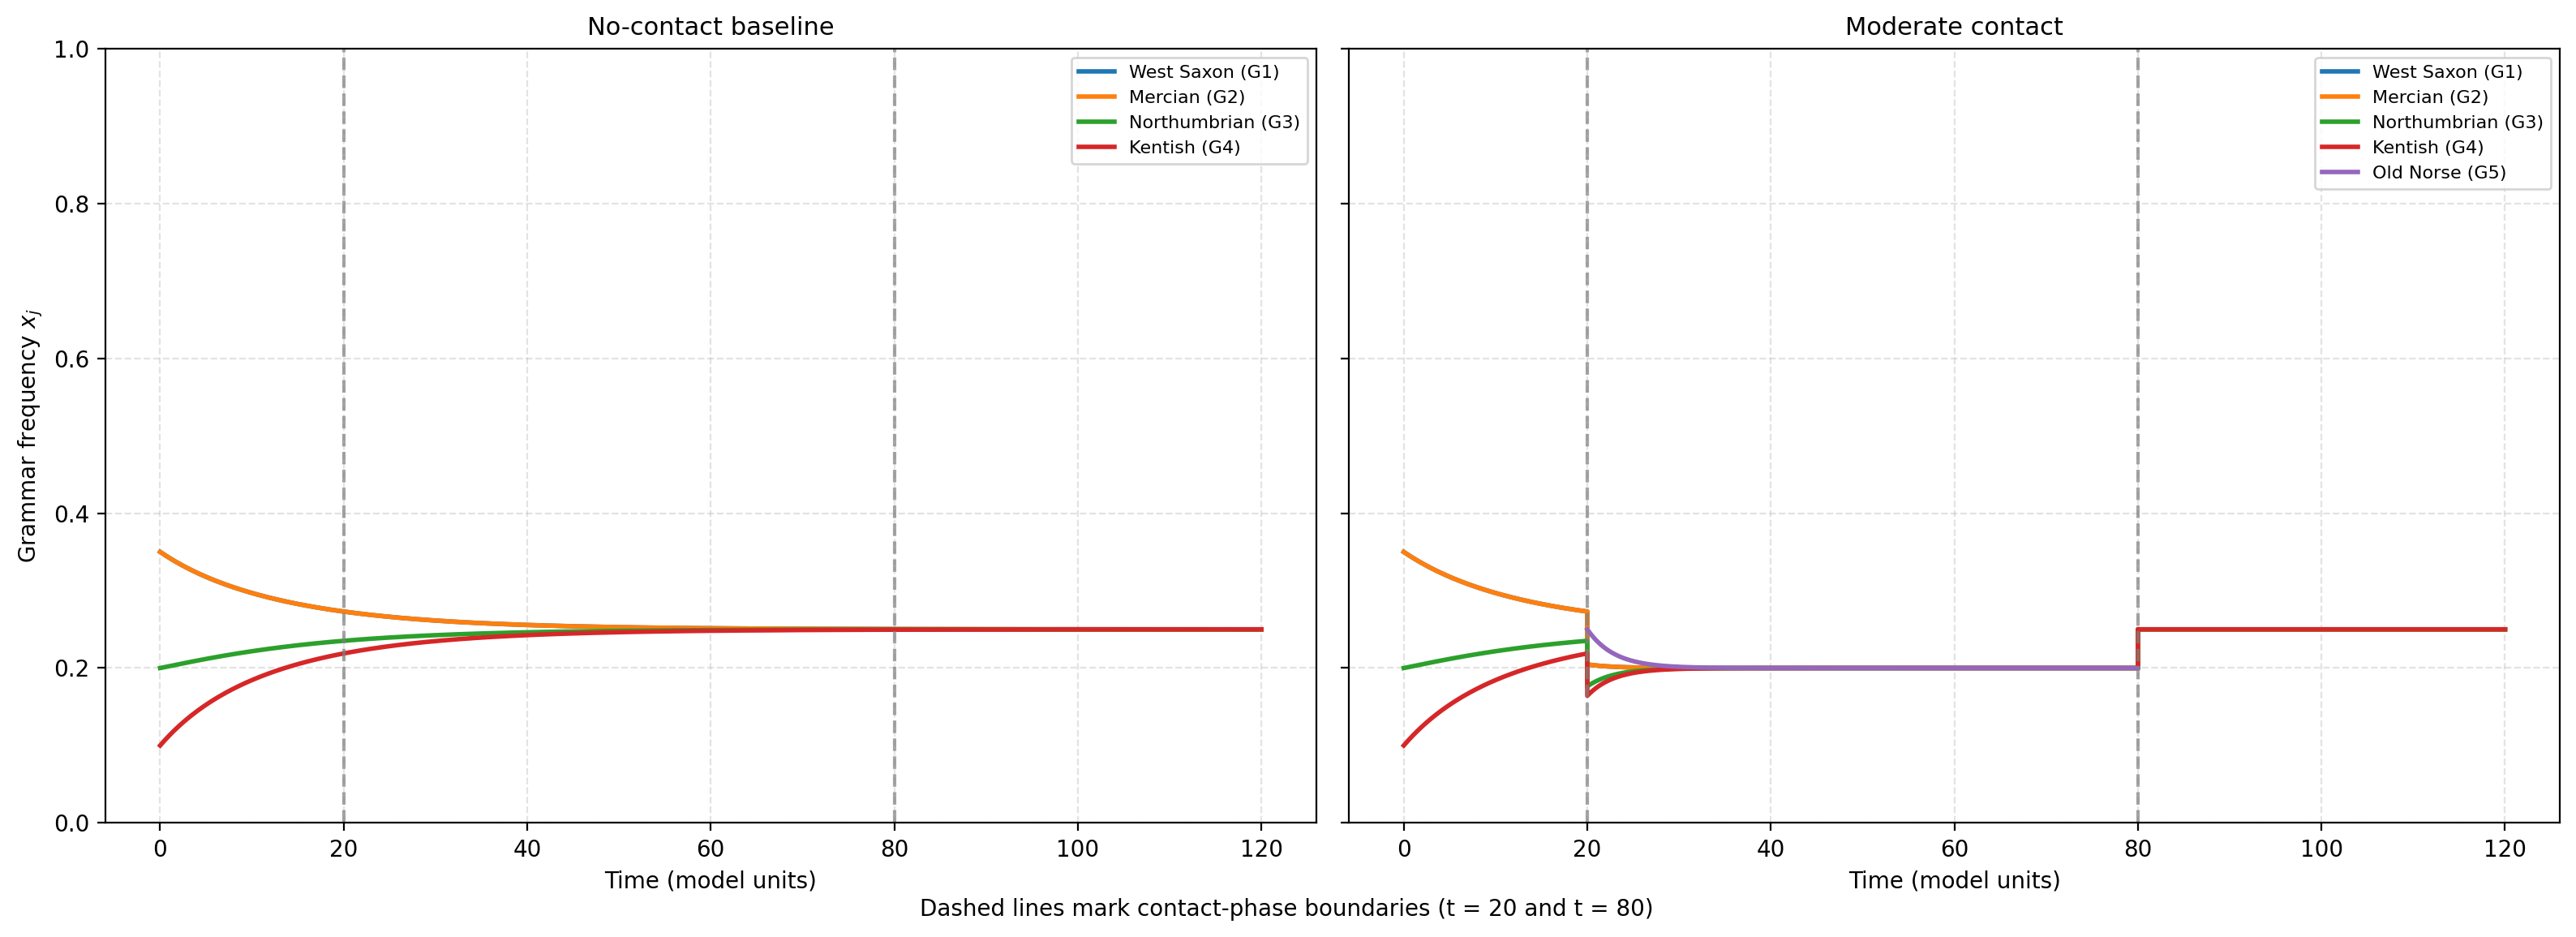
\includegraphics[width=\textwidth]{lde_comparison_nocontact_vs_moderate.png}
    \caption{Grammar frequency trajectories under no-contact (left) and moderate contact (right) scenarios. In the no-contact scenario, the four Old English components evolve under constant high learning fidelity with no additional grammar introduced ($n=4$ throughout). In the moderate contact scenario, the Old Norse component is introduced at the start of the contact phase (first dashed line) and removed at the end (second dashed line). The comparison illustrates the transient character of the contact perturbation: trajectories diverge from the no-contact baseline during the contact window and converge to the same near-uniform final state afterward.}
    \label{fig:comparison}
\end{figure}

Table~\ref{tab:displacement-integrals} quantifies this transient departure through the scalar integrals $D_H$ and $D_C$ defined in Equations~\eqref{eq:dH}--\eqref{eq:dC}. Consistent with the visual pattern in Figures~\ref{fig:scenario-entropy} and~\ref{fig:scenario-concentration}, the historically motivated scenarios show small normalized concentration displacements, while the strong and canonical scenarios produce larger departures. The canonical comparison produces the largest displacement because $a=0.50$ places the system nearer to Mitchener's coherent-equilibrium regime than the historically motivated high-$a$ scenarios. Raw $D_{M_2}$ is included only as a dimension-dependent diagnostic; it is strongly affected by the structural shift from $S_4$ to $S_5$ and should not be read as the primary scaling signal.

\begin{table}[h]
\centering
\caption{Transient displacement integrals computed by the trapezoid rule over $[0,120]$ model units using \texttt{compute\_transient\_displacement()} in \texttt{simulation.py}. $D_C$ is based on dimension-normalized concentration and is the primary concentration displacement metric. Raw $D_{M_2}$ is shown only to document the dimension-dependent diagnostic.}
\label{tab:displacement-integrals}
\small
\begin{tabular}{lccc}
\toprule
Scenario & $D_H$ & $D_C$ & Raw $D_{M_2}$ \\
\midrule
Canonical comparison  & 0.9912 & 0.8598 & 3.5129 \\
Conservative contact  & 0.0155 & 0.0135 & 3.0058 \\
Moderate contact      & 0.0170 & 0.0156 & 3.0095 \\
Strong contact        & 0.1747 & 0.1435 & 3.0691 \\
\bottomrule
\end{tabular}
\end{table}

\subsection{Ablation analysis}

The moderate contact scenario combines two interventions: a reduction in learning fidelity and the introduction of a fifth component. To separate these effects, Table~\ref{tab:ablation} compares four variants: a no-contact baseline, a $q$-shock-only run with $n=4$ throughout, a G5-injection-only run with $q=0.90$ throughout, and the combined contact run used in the main scenario. Figure~\ref{fig:ablation} shows the corresponding entropy and $C_n$ trajectories.

\begin{table}[h]
\centering
\caption{Ablation analysis for the moderate scenario. All values are generated by \texttt{simulation.py}. Raw $D_{M_2}$ is retained as a dimension-dependent diagnostic; $D_C$ is the comparable concentration displacement metric.}
\label{tab:ablation}
\scriptsize
\resizebox{\textwidth}{!}{%
\begin{tabular}{lcccccccc}
\toprule
Variant & Final entropy & Final $M_2$ & Final $C_4$ & $D_H$ & $D_C$ & Raw $D_{M_2}$ & Max mass error & Min. component \\
\midrule
No contact baseline & 1.0000 & 0.2500 & 0.0000 & 0.0000 & 0.0000 & 0.0000 & $2.22\times10^{-16}$ & 0.1000 \\
$q$-shock only & 1.0000 & 0.2500 & 0.0000 & 0.0186 & 0.0171 & 0.0128 & $8.22\times10^{-15}$ & 0.1000 \\
G5-injection only & 1.0000 & 0.2500 & 0.0000 & 0.0260 & 0.0189 & 2.9839 & $2.22\times10^{-16}$ & 0.1000 \\
Combined contact & 1.0000 & 0.2500 & 0.0000 & 0.0170 & 0.0156 & 3.0095 & $3.89\times10^{-15}$ & 0.1000 \\
\bottomrule
\end{tabular}%
}
\end{table}

\begin{figure}[h]
    \centering
    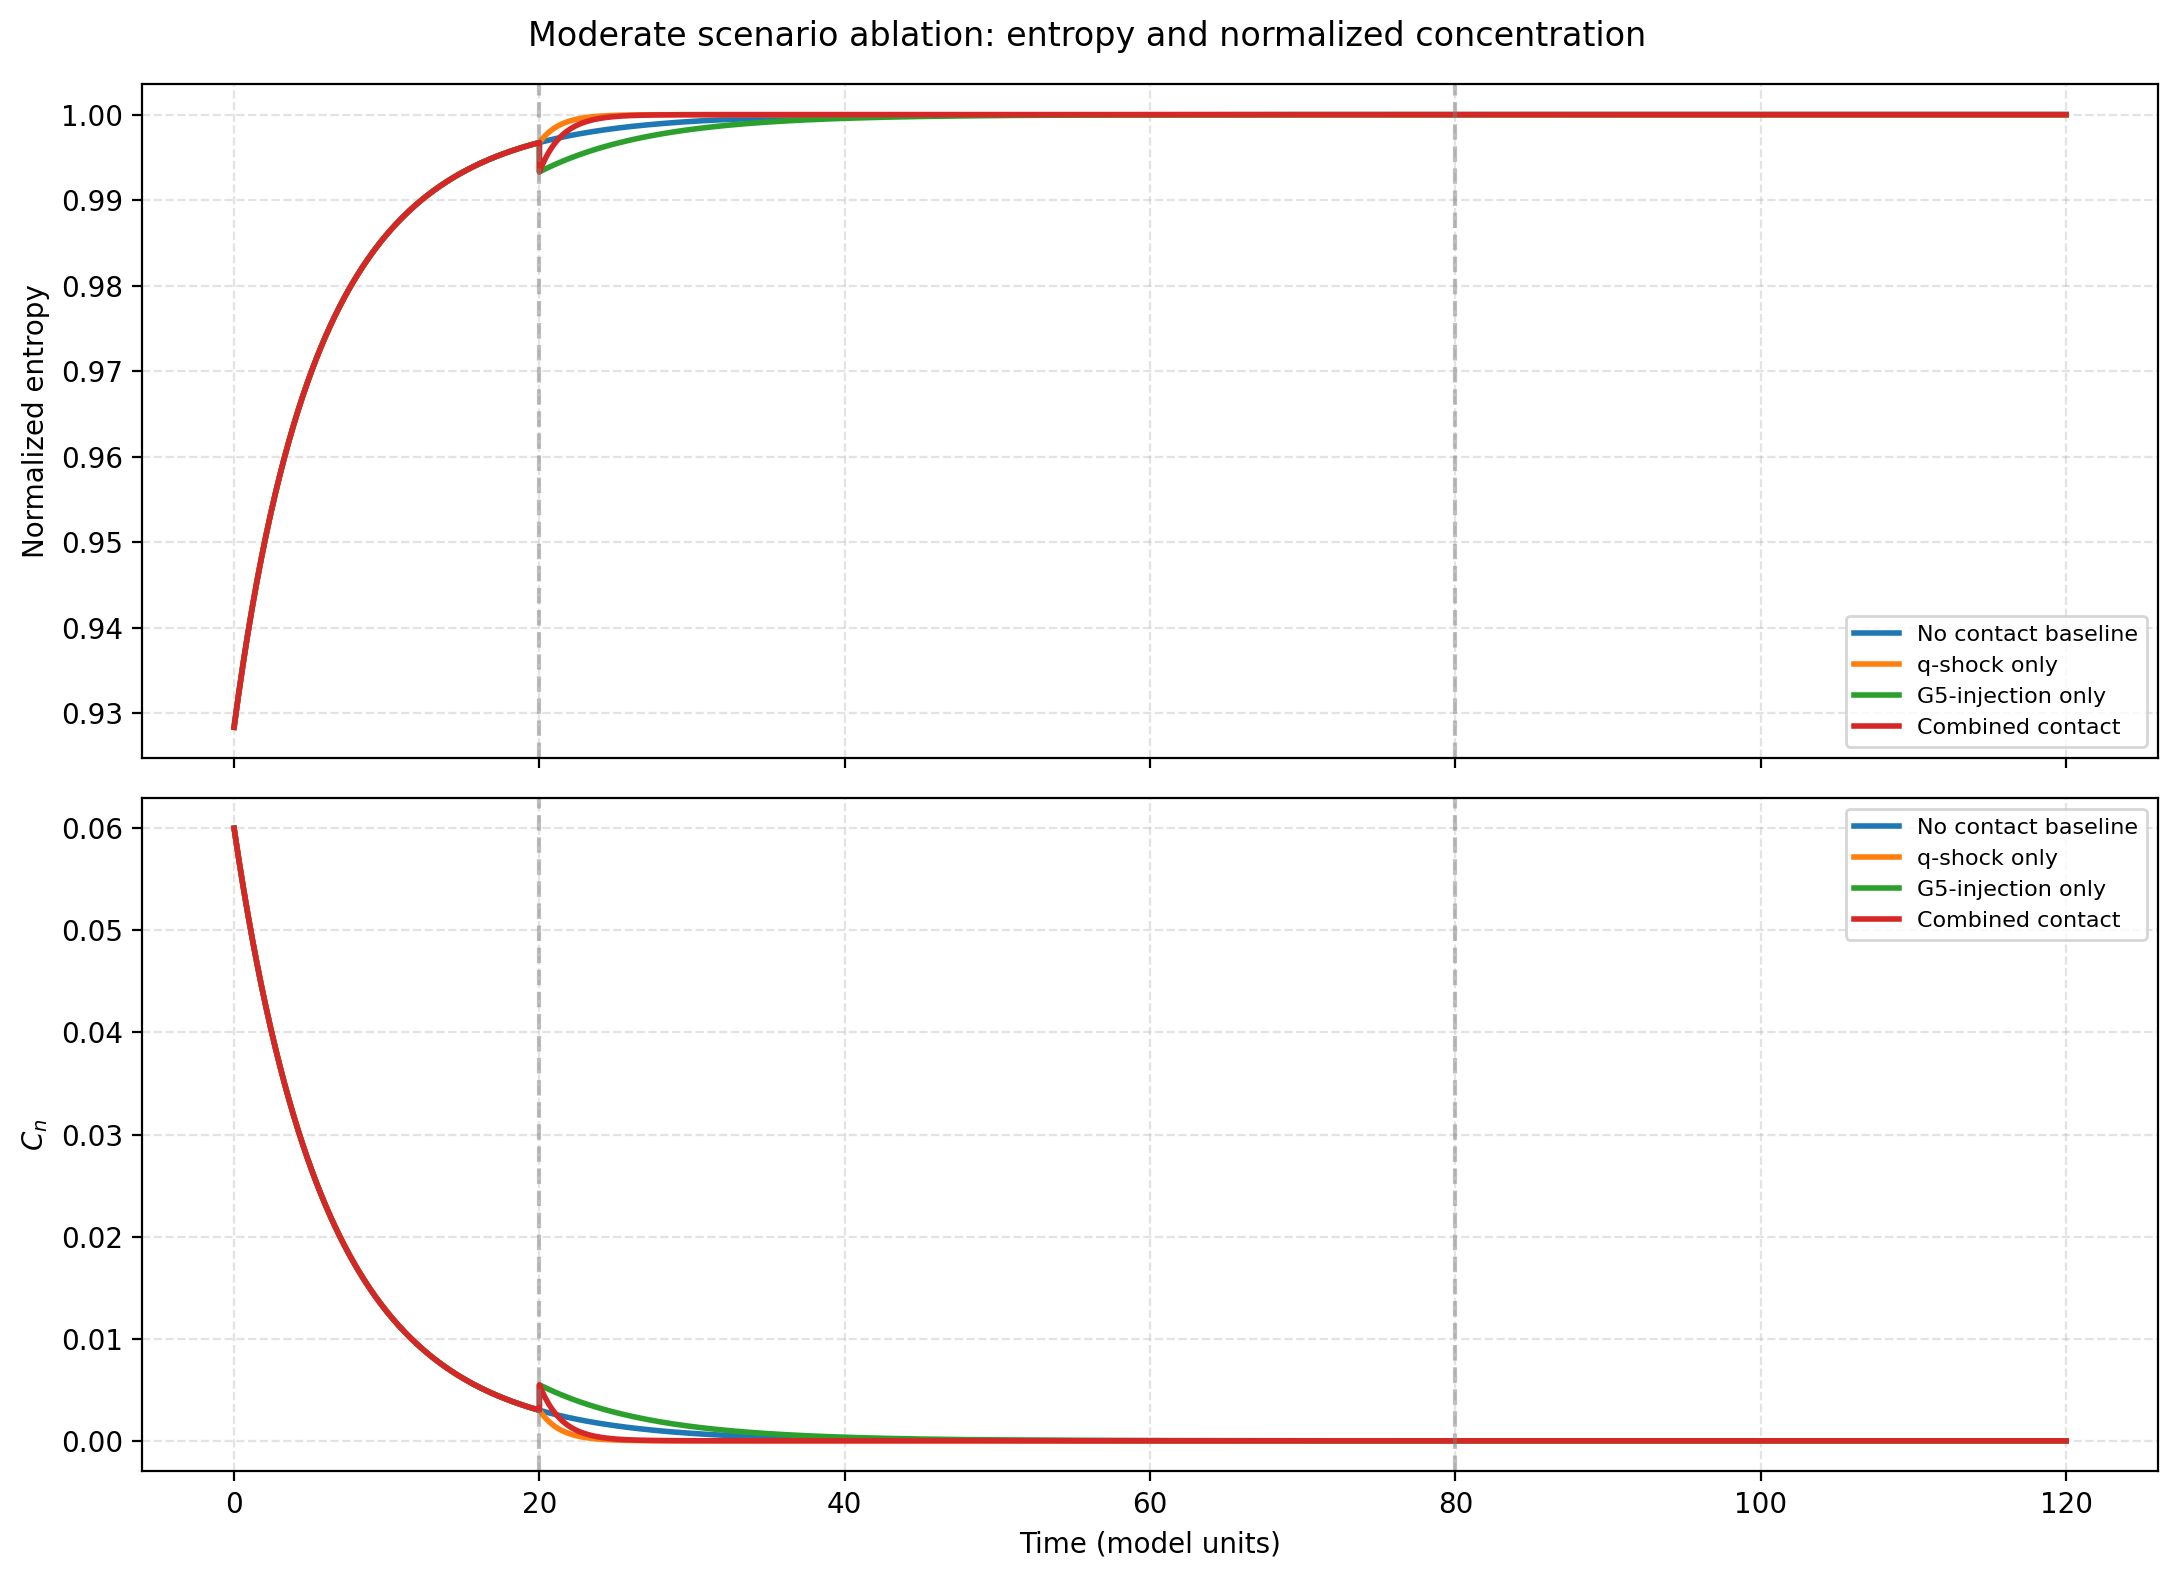
\includegraphics[width=0.9\textwidth]{lde_moderate_ablation_entropy_concentration.png}
    \caption{Ablation analysis for the moderate scenario. The $q$-shock-only and G5-injection-only variants isolate the learning-fidelity and component-insertion interventions. Differences are small in $D_C$ for the historically motivated moderate setting; raw $D_{M_2}$ is much larger for variants with a five-component phase because it is dimension-dependent.}
    \label{fig:ablation}
\end{figure}

\subsection{Redistribution sensitivity}
\label{sec:redistribution-sensitivity}

The main simulations use uniform redistribution of the Old Norse component at the end of contact. As a minimal sensitivity check, the moderate scenario was rerun with proportional redistribution, $\rho_i=y_i/\sum_{k=1}^4y_k$. The resulting diagnostics are numerically indistinguishable at the precision relevant here (Table~\ref{tab:redistribution}), and the trajectory-level comparison in Figure~\ref{fig:redistribution} shows no visible change in the main conclusion.

\begin{table}[h]
\centering
\caption{Sensitivity of the moderate scenario to the G5 redistribution rule.}
\label{tab:redistribution}
\small
\begin{tabular}{lccc}
\toprule
Redistribution rule & $D_H$ & $D_C$ & Raw $D_{M_2}$ \\
\midrule
Uniform & 0.0170 & 0.0156 & 3.0095 \\
Proportional & 0.0170 & 0.0156 & 3.0095 \\
\bottomrule
\end{tabular}
\end{table}

\begin{figure}[h]
    \centering
    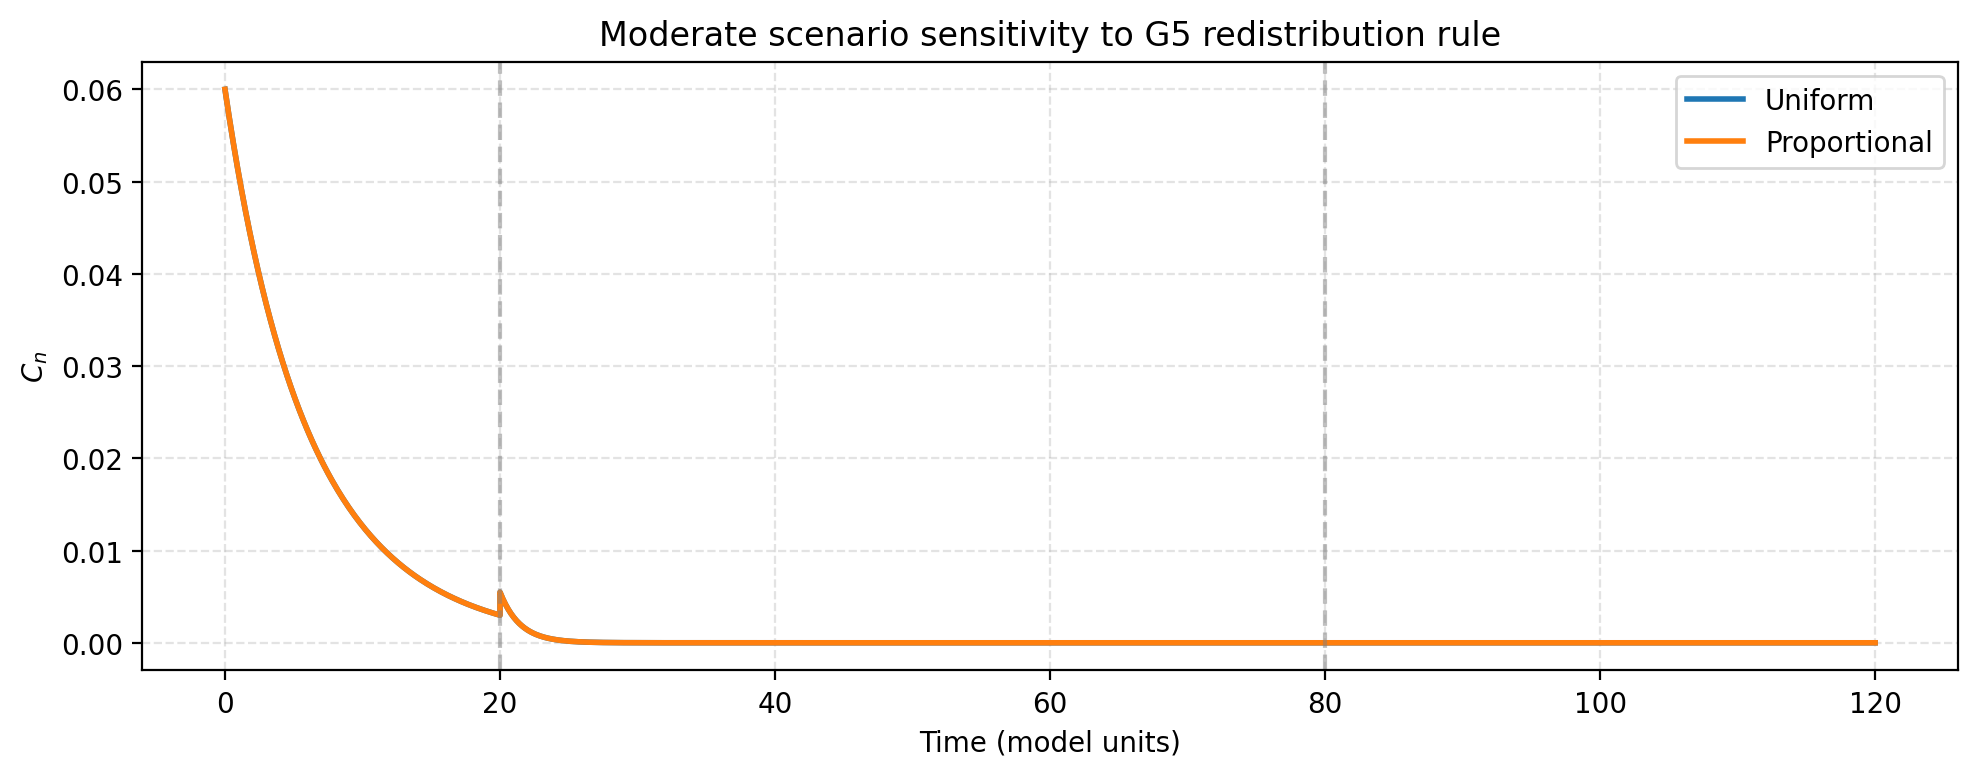
\includegraphics[width=0.85\textwidth]{lde_redistribution_sensitivity.png}
    \caption{Moderate-scenario sensitivity to the end-of-contact redistribution rule. Uniform and proportional redistribution give visually overlapping $C_n$ trajectories in this symmetric setting. This should not be read as a general historical claim; asymmetric or regionally informed redistribution rules remain future work.}
    \label{fig:redistribution}
\end{figure}

\subsection{Parameter sweep}

A sweep over $(a,q_2)$ locates the historically motivated scenarios within the full parameter space and identifies the regions in which qualitatively different final-state behavior emerges. This is important because the canonical bifurcation analysis in \citet{mitchener2003bifurcation} operates near $a=0.5$, where coherent equilibria are accessible at sufficiently high $q$. The historically motivated scenarios use higher values of $a$ (0.75--0.80), reflecting a modelling assumption of relatively high cross-grammar intelligibility among related Germanic varieties. As Figure~\ref{fig:heatmap} shows, this places the portfolio in a parameter region where final normalized concentration remains close to zero. Final-state concentration increases mainly in the low-$a$, high-$q_2$ region, where cross-grammar intelligibility is low and learning fidelity remains sufficiently high to support concentration around fewer grammars. Lower $q_2$ strengthens the mutation-like term and tends to push the system toward the uniform state.

\begin{figure}[h]
    \centering
    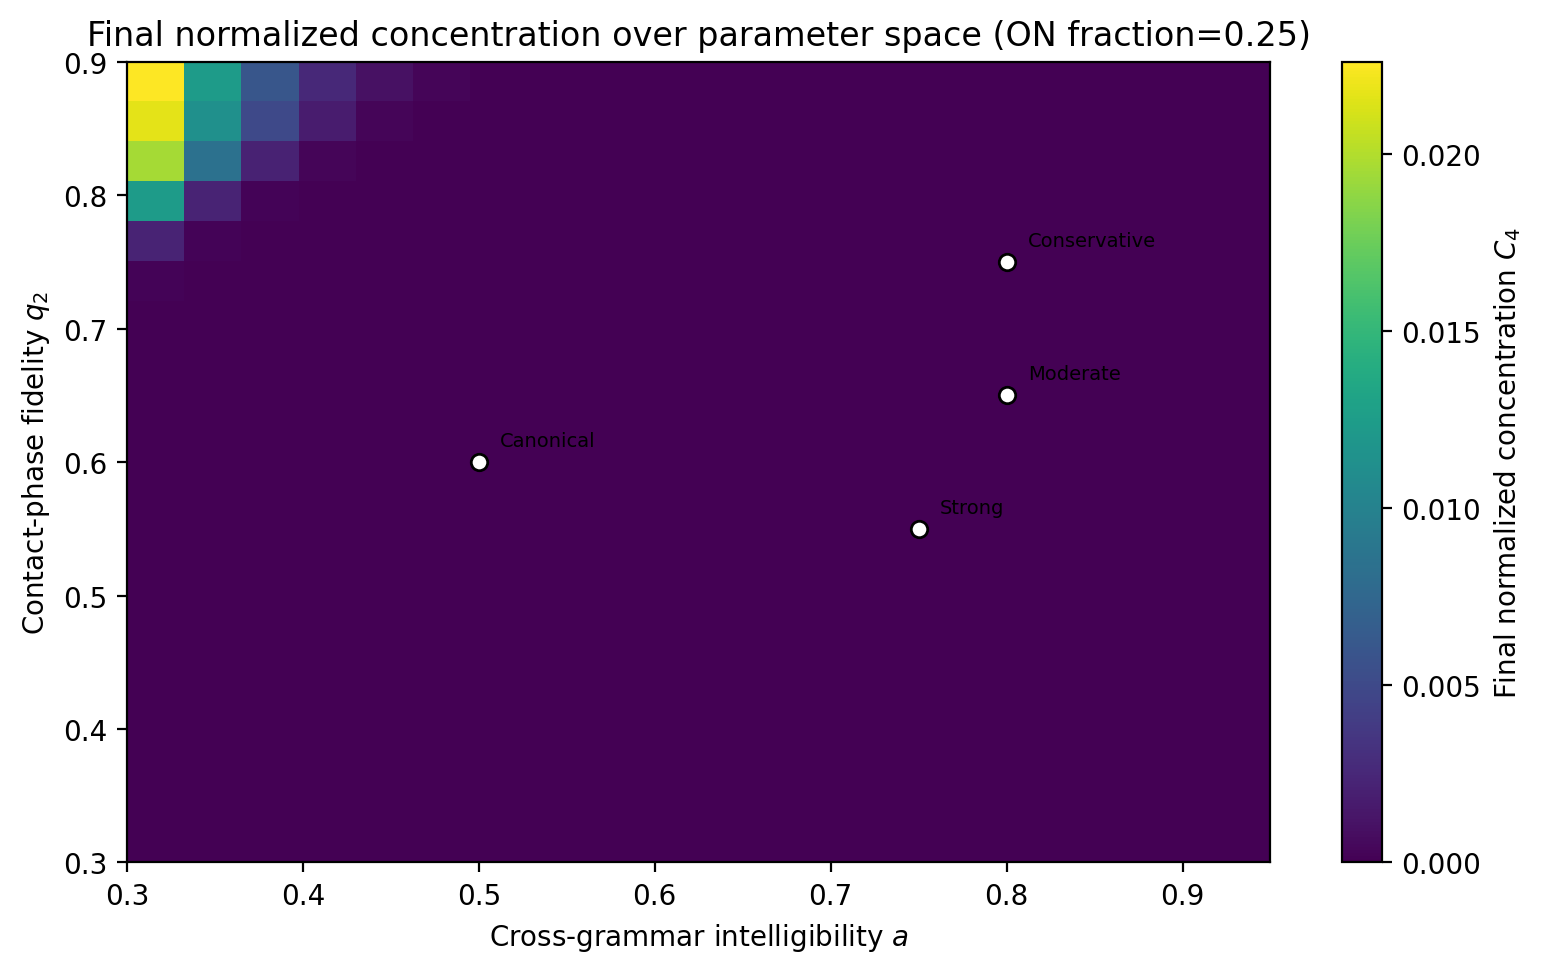
\includegraphics[width=0.85\textwidth]{lde_heatmap_final_c.png}
    \caption{Heatmap of final normalized concentration $C_4$ under variation of average intelligibility $a$ and contact-phase learning fidelity $q_2$ for a fixed Old Norse contact intensity $\theta=0.25$. Scenario markers show the $(a,q_2)$ coordinates of the conservative, moderate, strong, and canonical comparison runs. Final-state concentration increases mainly in the low-$a$, high-$q_2$ region; lowering $q_2$ strengthens the mutation-like term and tends to push trajectories toward the uniform state.}
    \label{fig:heatmap}
\end{figure}

\section{Discussion}

The simulations illustrate how the symmetric language dynamical equation responds to contact-like perturbations. In the historically motivated parameter regime used here---average intelligibility $a \in [0.75, 0.80]$, contact-phase fidelity $q_2 \in [0.55, 0.75]$---all scenarios converge to the same near-uniform final state. The effect of contact is therefore transient rather than asymptotic: the reduction in $q$ and the temporary fifth component push the system toward a more distributed configuration during the contact window, but the trajectories return to the same four-component uniform attractor. This is consistent with the mechanism described in \citet{mitchener2003bifurcation}, but it is weaker than a claim that contact destabilizes a coherent pre-contact equilibrium.

The local threshold calculation clarifies why this qualification matters. For $a=0.80$ and $a=0.75$, the critical fidelities for the uniform equilibrium in $S_4$ are approximately 0.9583 and 0.9464, respectively. The historically motivated scenarios begin at $q_1=0.90$, below these thresholds, so they already lie in a regime where the uniform equilibrium is locally stable. These scenarios therefore show measurable transient displacement within a uniform-attractor regime, not strong bifurcation-driven instability. The canonical comparison with $a=0.50$ is different: $q_c=0.875$, so $q_1=0.90$ lies closer to the coherent-equilibrium side of Mitchener's bifurcation structure. This explains why the canonical comparison has larger displacement, but it remains a methodological reference rather than a historical calibration.

The heatmap (Figure~\ref{fig:heatmap}) also revises the interpretation of final-state divergence. Stronger final concentration emerges mainly in the low-$a$, high-$q_2$ region, where cross-grammar intelligibility is low and learning fidelity remains high enough to permit concentration around fewer grammars. Low $q_2$ does not create this final concentration; it strengthens the mutation-like learning-error term and tends to push the system toward the uniform state.

However, the interpretation must remain cautious. The components $G_1,\ldots,G_5$ are idealized grammatical systems, not directly observed populations. The parameters $q$, $a$, and the Old Norse fraction are not historical measurements. The model does not track specific grammatical features such as case loss, word order change, or agreement morphology. Therefore, it cannot establish that Old Norse contact caused Middle English simplification. It can only show that, within this mathematical framework, reduced learning fidelity and contact-component insertion have the right qualitative form to produce transient displacement in the grammar distribution.

The main value of the model is thus exploratory. It offers a transparent way to formalize assumptions about learning reliability, contact, and grammatical competition, and to test whether qualitative outcomes are robust under parameter variation. Future work should connect the parameters to corpus-based proxies and should explore asymmetric intelligibility matrices.

\section{Limitations}

This study has several important limitations.

\begin{enumerate}
    \item \textbf{Symmetric intelligibility.} The model assumes a single value $a$ for all cross-grammar intelligibility relations. This is unrealistic for Old English dialects and Old Norse, but it preserves comparability with Mitchener's analytical framework.
    \item \textbf{Heuristic parameters.} The parameters are scenario values, not measurements. They must be supported by historical arguments and sensitivity analysis rather than treated as facts.
    \item \textbf{Discrete phase maps.} The transition maps $\mathcal I_\theta$ and $\mathcal R_\rho$ are modelling devices, not historical processes. The uniform redistribution rule is neutral and reproducible, but it is not a reconstruction of post-contact regional assimilation. Future work could use proportional, regional, or corpus-informed redistribution rules in asymmetric models.
    \item \textbf{No direct corpus calibration.} The present version does not estimate parameters from corpora. Corpus resources may provide indirect proxies in future work.
    \item \textbf{No spatial structure.} The model assumes a freely interacting population, whereas historical language contact was geographically structured.
    \item \textbf{No feature-level grammar.} The model tracks idealized grammar frequencies but does not represent particular morphosyntactic features.
\end{enumerate}

\section{Conclusion}

This paper reinterprets the Old-to-Middle English transition as a computational case study for the symmetric language dynamical equation. Rather than proposing a new mathematical model or claiming to reconstruct historical demographics, it implements historically motivated scenarios suggested by Mitchener's discussion of Scandinavian contact. The resulting simulations show that a contact phase can produce measurable transient displacement in model-state diversity and concentration, even when the long-run attractor remains unchanged. The scalar displacement integrals $D_H$ and $D_C$ provide a compact quantitative summary of this transient effect across scenarios. The findings support the use of dynamical models as exploratory tools for historical linguistics, provided their assumptions are made explicit and their parameters are treated as scenario-based rather than directly observed.

Future work should strengthen the historical grounding with page-level primary-source references, corpus-informed proxies, and asymmetric intelligibility matrices.

\section*{Code Availability}

All simulation code is publicly available at the project repository:
\begin{center}
\url{https://github.com/cmorregof/language_dynamics}
\end{center}
The repository includes the main Python script, dependencies, and generated figures.

\section*{Declaration on AI-Assisted Tools}
Claude (Anthropic) was used in an assistive capacity for:
\begin{itemize}
    \item Language editing and grammar checking (no changes to scientific content or conclusions)
    \item Python code review for syntax and efficiency (no changes to algorithms or numerical methods)
    \item Literature organization and research planning
\end{itemize}
All mathematical derivations, numerical implementation, parameter choices, result interpretation, and conclusions are the sole work of the authors. The authors manually checked the bibliographic entries and the way each source is used in the manuscript.

\begin{thebibliography}{99}

\bibitem[Abrams and Strogatz(2003)]{abramsstrogatz2003language}
Abrams, D. M., \& Strogatz, S. H. (2003). Modelling the dynamics of language death. \textit{Nature}, 424, 900. \url{https://doi.org/10.1038/424900a}

\bibitem[Castellano et~al.(2009)]{castellano2009statistical}
Castellano, C., Fortunato, S., \& Loreto, V. (2009). Statistical physics of social dynamics. \textit{Reviews of Modern Physics}, 81(2), 591--646. \url{https://doi.org/10.1103/RevModPhys.81.591}

\bibitem[Eigen(1971)]{eigen1971selforganization}
Eigen, M. (1971). Selforganization of matter and the evolution of biological macromolecules. \textit{Naturwissenschaften}, 58, 465--523.

\bibitem[Komarova et~al.(2001)]{komarova2001grammar}
Komarova, N. L., Niyogi, P., \& Nowak, M. A. (2001). The evolutionary dynamics of grammar acquisition. \textit{Journal of Theoretical Biology}, 209(1), 43--59. \url{https://doi.org/10.1006/jtbi.2000.2240}

\bibitem[Kauhanen(2020)]{kauhanen2021replicator}
Kauhanen, H. (2020). Replicator--mutator dynamics of linguistic convergence and divergence. \textit{Royal Society Open Science}, 7(11), 201682. \url{https://doi.org/10.1098/rsos.201682}

\bibitem[Kauhanen(2022)]{kauhanen2022bifurcation}
Kauhanen, H. (2022). A bifurcation threshold for contact-induced language change. \textit{Glossa: A Journal of General Linguistics}, 7(1), Article 10, 1--32. \url{https://doi.org/10.16995/glossa.8211}

\bibitem[Mitchener(2003)]{mitchener2003bifurcation}
Mitchener, W. G. (2003). Bifurcation analysis of the fully symmetric language dynamical equation. \textit{Journal of Mathematical Biology}, 46, 265--285. \url{https://doi.org/10.1007/s00285-002-0172-8}

\bibitem[Mitchener and Nowak(2003)]{mitchenernowak2003competitive}
Mitchener, W. G., \& Nowak, M. A. (2003). Competitive exclusion and coexistence of universal grammars. \textit{Bulletin of Mathematical Biology}, 65(1), 67--93. \url{https://doi.org/10.1006/bulm.2002.0322}

\bibitem[Mitchener(2007)]{mitchener2007game}
Mitchener, W. G. (2007). Game dynamics with learning and evolution of universal grammar. \textit{Bulletin of Mathematical Biology}, 69(3), 1093--1118. \url{https://doi.org/10.1007/s11538-006-9165-x}

\bibitem[Mira and Paredes(2005)]{mira2005interlinguistic}
Mira, J., \& Paredes, A. (2005). Interlinguistic similarity and language death dynamics. \textit{Europhysics Letters}, 69(6), 1031--1034. \url{https://doi.org/10.1209/epl/i2004-10438-4}

\bibitem[Niyogi and Berwick(1997)]{niyogi1997dynamical}
Niyogi, P., \& Berwick, R. C. (1997). A dynamical systems model for language change. \textit{Complex Systems}, 11(3), 161--204.

\bibitem[Niyogi and Berwick(2009)]{niyogi2009proper}
Niyogi, P., \& Berwick, R. C. (2009). The proper treatment of language acquisition and change in a population setting. \textit{Proceedings of the National Academy of Sciences}, 106(25), 10124--10129. \url{https://doi.org/10.1073/pnas.0903993106}

\bibitem[Baugh and Cable(2012)]{baugh2012history}
Baugh, A. C., \& Cable, T. (2012). \textit{A History of the English Language} (6th ed.). Routledge.

\bibitem[Dawson(2003)]{dawson2003defining}
Dawson, H. C. (2003). Defining the outcome of language contact: Old English and Old Norse. \textit{Ohio State University Working Papers in Linguistics}, 57, 40--57.

\bibitem[Thomason and Kaufman(1988)]{thomasonkaufman1988contact}
Thomason, S. G., \& Kaufman, T. (1988). \textit{Language Contact, Creolization, and Genetic Linguistics}. University of California Press.

\bibitem[Gneuss(1972)]{gneuss1972standard}
Gneuss, H. (1972). The origin of Standard Old English and \AE thelwold's school at Winchester. \textit{Anglo-Saxon England}, 1, 63--83.

\bibitem[Gretsch(2001)]{gretsch2001winchester}
Gretsch, M. (2001). Winchester vocabulary and Standard Old English. \textit{Bulletin of the John Rylands Library}, 83(1), 41--87.

\bibitem[Hofstetter(1988)]{hofstetter1988winchester}
Hofstetter, W. (1988). Winchester and the standardization of Old English vocabulary. \textit{Anglo-Saxon England}, 17, 139--168.

\bibitem[Hogg(1992)]{hogg1992cambridge}
Hogg, R. M. (Ed.). (1992). \textit{The Cambridge History of the English Language, Volume I: The Beginnings to 1066}. Cambridge University Press.

\bibitem[Kershaw and R{\o}yrvik(2016)]{kershawroyvik2016people}
Kershaw, J., \& R{\o}yrvik, E. C. (2016). The ``People of the British Isles'' project and Viking settlement in England. \textit{Antiquity}, 90(354), 1670--1680.

\bibitem[Raffield(2020)]{raffield2020danelaw}
Raffield, B. (2020). The Danelaw reconsidered: Colonization and conflict in Viking-Age England. \textit{Viking and Medieval Scandinavia}, 16, 181--220.

\bibitem[Townend(2002)]{townend2002language}
Townend, M. (2002). \textit{Language and History in Viking Age England: Linguistic Relations between Speakers of Old Norse and Old English}. Brepols.

\bibitem[Pons-Sanz(2013)]{pons-sanz2013lexical}
Pons-Sanz, S. M. (2013). \textit{The Lexical Effects of Anglo-Scandinavian Linguistic Contact on Old English}. Brepols.

\bibitem[Walkden et~al.(2023)]{walkden2023sociolinguistic}
Walkden, G., McCarley, G. H., Montero, R., Rolf, M., Einhaus, S., \& Kauhanen, H. (2023). Sociolinguistic typology meets historical corpus linguistics. \textit{Transactions of the Philological Society}, 121(3), 546--567.

\bibitem[Warner(2017)]{warner2017english}
Warner, A. (2017). English--Norse contact, simplification, and sociolinguistic typology. \textit{Neuphilologische Mitteilungen}, 118(2), 317--404.

\end{thebibliography}

\end{document}
